\chapter{Umsetzung des Prototyps}\label{sec:realisation}

Nachdem in Kapitel \ref{sec:concept} die Konzeption der Anwendungen dargestellt wurde, folgt in diesem Kapitel die Beschreibung der praktischen Umsetzung.

Zunächst wird die Ausgangssituation erläutert, wie sie sich aus dem vorangegangenen Projekt ergab. Anschließend erfolgt eine Übersicht der verwendeten Technologien. Darauf aufbauend werden die entwickelten Anwendungen im Detail vorgestellt. Abschließend werden zentrale Herausforderungen und Probleme beschrieben, die im Verlauf der Umsetzung auftraten.

\section{Ausgangssituation}

In der vorangegangenen Arbeit wurde ein erstes funktionsfähiges \ac{MVP} der Spielidee realisiert das sich aus drei Hauptkomponenten zusammensetzt. Die Spielanwendung für den Player wurde mithilfe der Game Engine Unity umgesetzt. Das Spielgeschehen des Watchers wurde hingegen als Webanwendung auf Basis des Vue3-Frameworks realisiert. Für die Kommunikation zwischen beiden Anwendungen wurde ein WebSocket-Server auf Grundlage von Express.js (Auf Basis von Node.js) entwickelt. Dieser Server steht zusätzlich in Verbindung mit einer MongoDB-Datenbank, in der die Fortschritte einzelner Spielsessions gespeichert werden.

Die Anwendungen des Players und des Watchers fungieren in diesem System als visuelle und interaktive Frontend, die auf Nutzereingaben reagieren. Diese Eingaben werden an den Server übermittelt, der sie zur Laufzeit verarbeitet und bei Bedarf persistent in der Datenbank speichert.

\subsection{Aufbau der Ausgangssituation}

Im Softwaredesign wurde in diesem Zusammenhang häufig auf das \ac{MVC} zurückgegriffen (vgl. \citealp{GlossarWiki:Reenskaug:1979a}). Das Modell (Model) definiert die Datenstruktur der Anwendung und enthält die zugrunde liegende Information. Bei einer Zustandsänderung benachrichtigt das Modell die jeweiligen Views, sodass die Darstellung der Daten entsprechend aktualisiert wird. In einigen Implementierungen wird zusätzlich auch das Controller über Änderungen informiert.

Die View legt fest, wie die Daten visuell präsentiert werden. Der Controller wiederum ist für die Bearbeitung der Nutzereingabe verantwortlich. Er nimmt die Änderungen aus der View entgegen und übermittelt sie entweder an das Modell oder direkt zurück an die View (vgl. \citealp{noauthor_mvc_2023}, Abbildung \ref{fig:mvc-diagramm}).

\begin{figure}[ht]
\centering
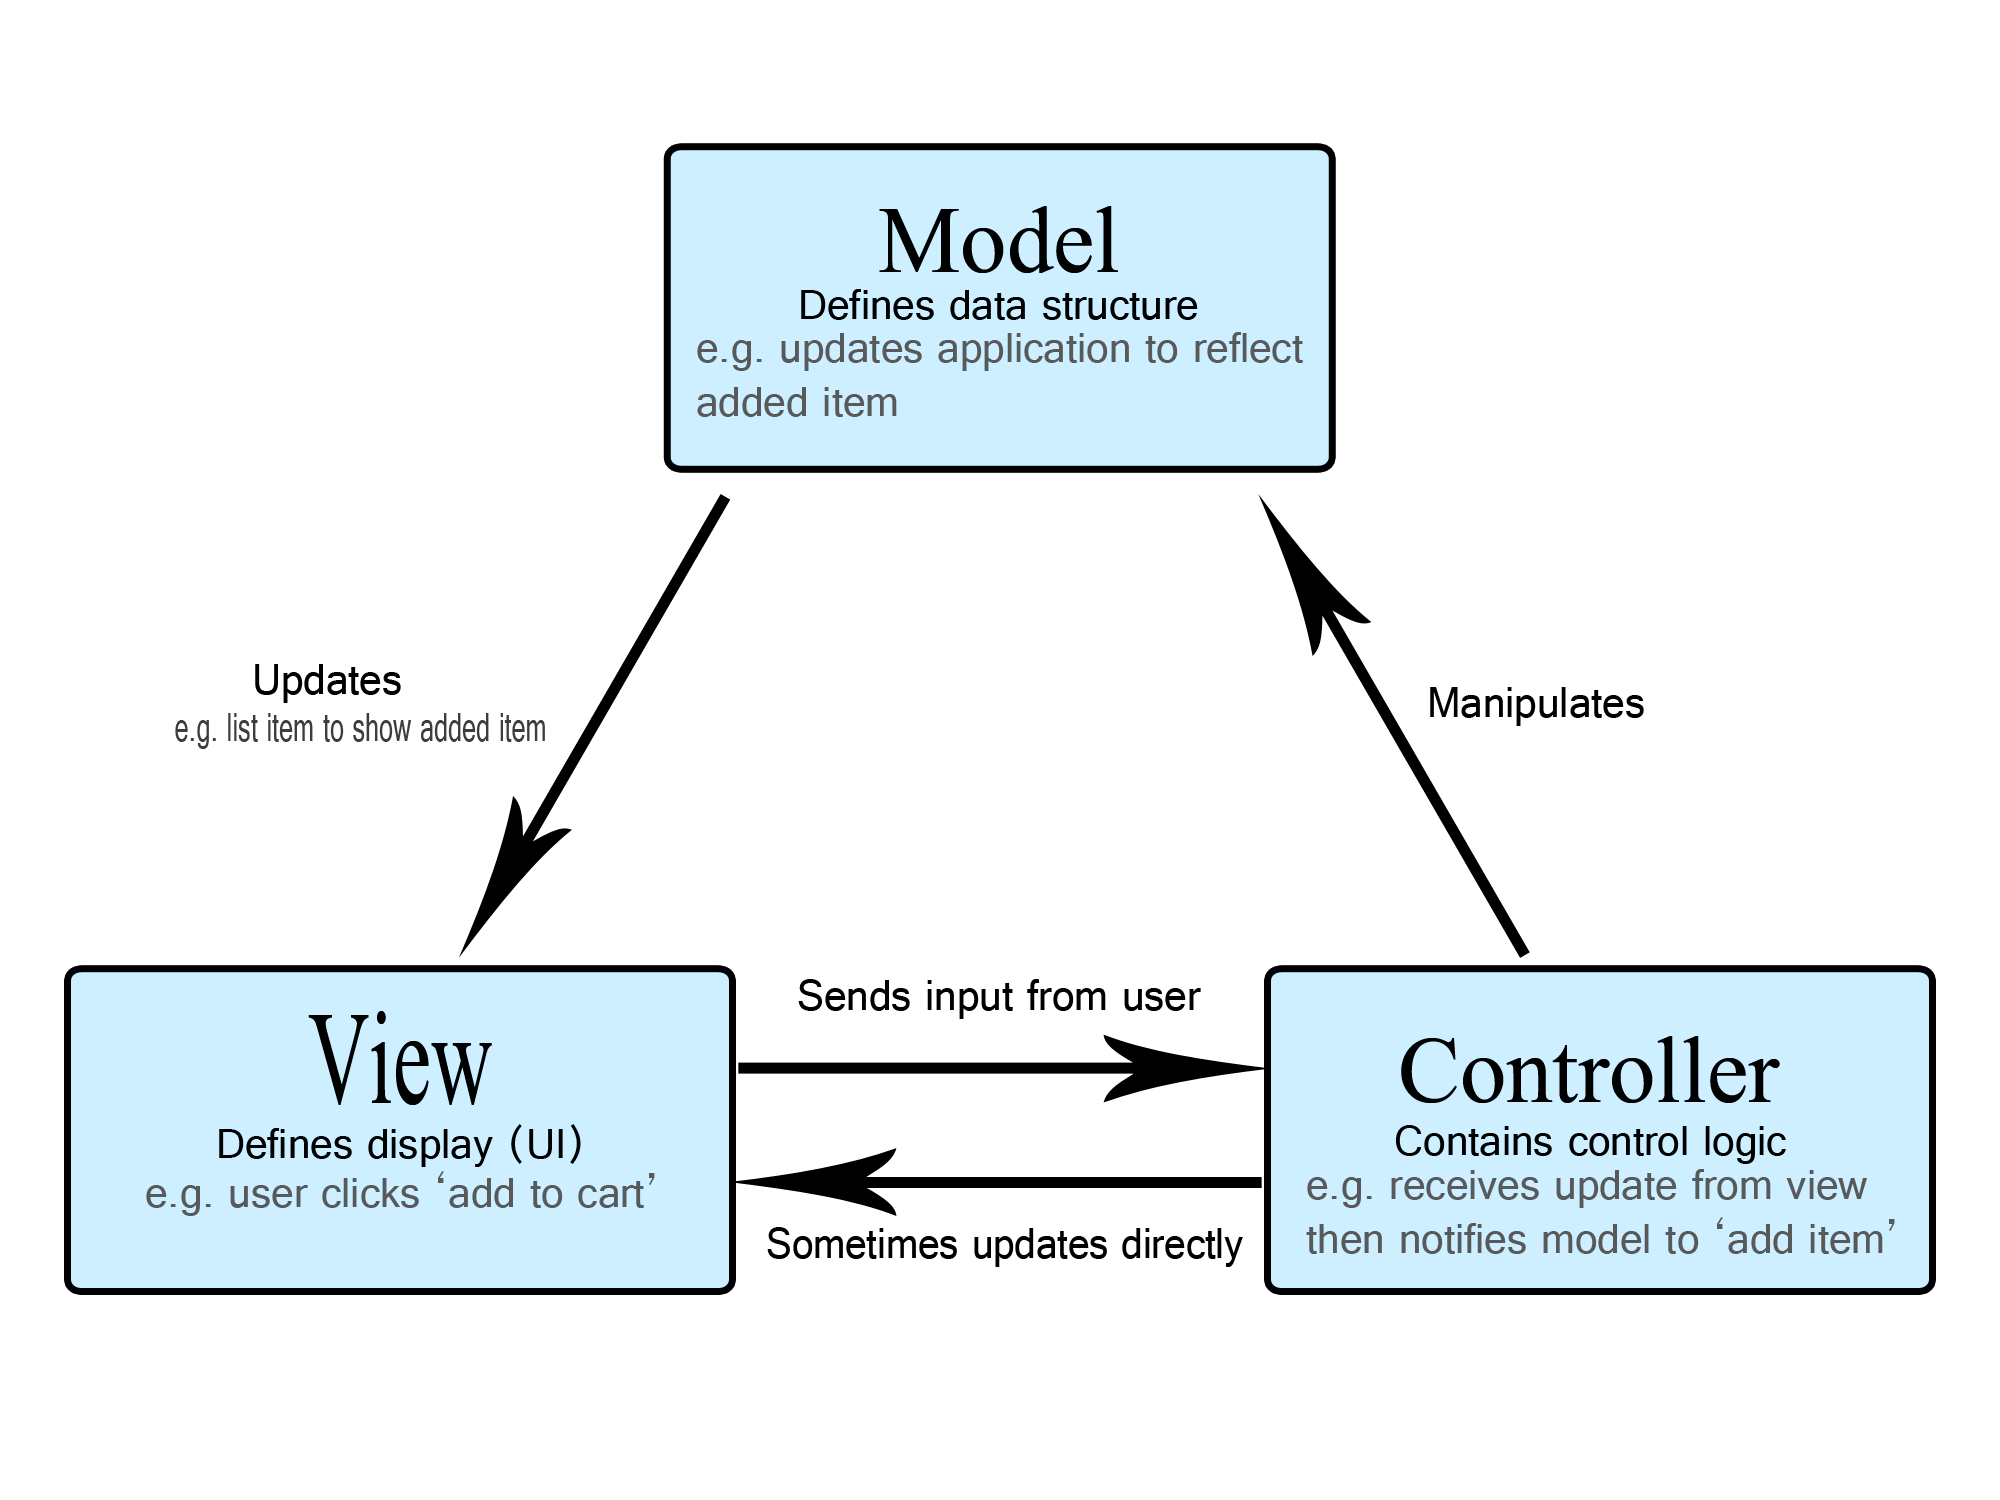
\includegraphics[width=1\linewidth]{content/pictures/mvc-architecture.png}
\caption{\ac{MVC} Beispiel-Diagramm (Quelle: \cite{noauthor_mvc_2023})}
\label{fig:mvc-diagramm}
\end{figure}

Innerhalb der Systemarchitektur übernehmen die MongoDB-Datenbank sowie bestimmte Klassen des WebSocket-Servers die Rolle des Modells. Sie verwalten die zentralen Anwendungsdaten und deren Persistenz. Die verschiedenen WebSocket-Nachrichtenendpunkte fungieren als Controller. Sie verarbeiten eingehende Nachrichten, koordinieren die Datenflüsse zwischen Modul und View und steuern die Anwendungslogik. Die \say{Frontends} der Watcher- und Player-Anwendungen bilden die Views des \ac{MVC}-Design-Patterns und dienen der Darstellung sowie Interaktion mit dem Nutzer.

\subsection{Beitreten einer Session}

\begin{figure}[ht]
\centering
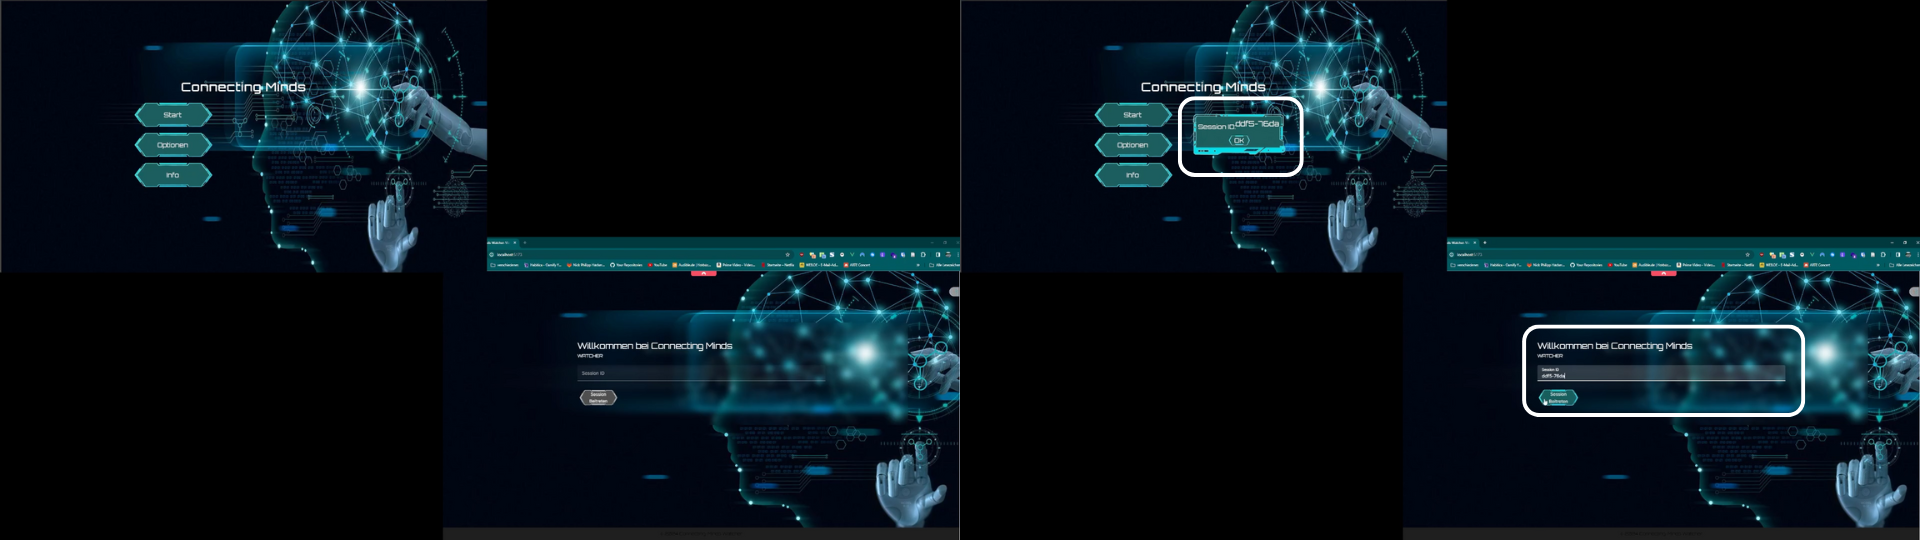
\includegraphics[width=1\linewidth]{content/pictures/Login_Login_by_ID.png}
\caption{Startbildschirme der Player und Watcher Anwendung (Quelle: eigene Darstellung)}
\label{fig:old-logins}
\end{figure}

Abbildung \ref{fig:old-logins} zeigt den bereits im früheren Prototyp entwickelten Startbildschirm, über den der Player eine neue Spielsession starten (linkes Bild, oben links) und der Watcher dieser beitreten kann (linkes Bild, unten rechts). Nachdem der Player eine Session erstellt hat, erhält er vom WebSocket-Server eine Rückmeldung mit der dazugehörigen Session-ID (rechtes Bild, oben links). Diese ID muss er dem Watcher mitteilen, damit dieser der entsprechenden Session beitreten kann (rechtes Bild, unten rechts).

\subsection{Einführung in die Anwendungen}

\begin{figure}[ht]
\centering
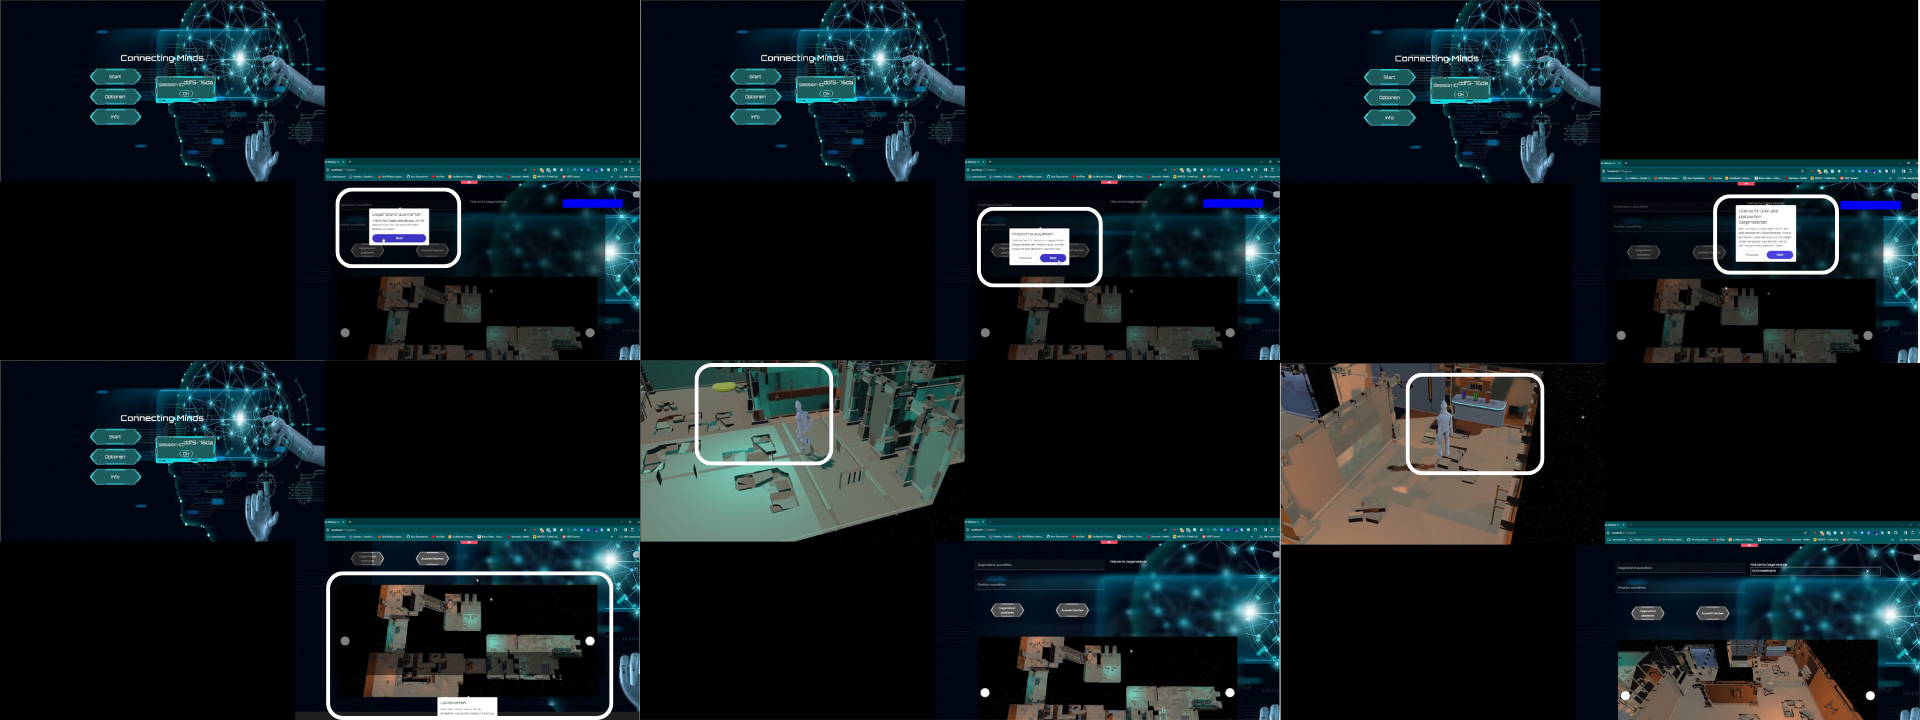
\includegraphics[width=1\linewidth]{content/pictures/Introduction.png}
\caption{Einführung in die Anwendung des Players und Watchers (Quelle: eigene Darstellung)}
\label{fig:old-introductions}
\end{figure}

Abbildung \ref{fig:old-introductions} zeigt die Einführung der beiden Anwendungen in die Spielwelt. Zu Beginn erhält der Watcher verschiedene Tooltips, die ihm die Grundfunktionen seiner Anwendung erläutern (vgl. erstes bis drittes Bild in der ersten Zeile und linkes Bild in der zweiten Zeile; jeweils in weiß umrandet im rechten Bildelement). Die Anwendung des Watchers umfasst zwei Dropdown-Menüs, über die Gegenstände und deren Positionen ausgewählt werden können (erste Zeile, Bilder links und und in der Mitte), eine Lister aller aktuell platzierten Objekte (erste Zeile rechts Bild), welche einzeln wieder entfernt werden können, sowie eine Top-Down-Ansicht der Spielwelt, in der sich der Player befindet (zweite Zeile, linkes Bild). 

Der Player steuert seinen Avatar durch Antippen der gewünschten Position auf dem Bildschirm (zweite Reihe mittlere Bild, linkes Bildelement). Zusätzlich kann er die Kamerahöhe in Relation zur Spielfigur durch vertikale Wischbewegungen (Swipes) anpassen, wodurch sich die Perspektive innerhalb eines bestimmten Rahmens verändert.

Um das gemeinsame Spielziel zu erreichen, müssen Player und Watcher kooperieren und gemeinsam Hindernisse in der Spielwelt überwinden. Ein solches Rätselelement, das im Zusammenspiel gelöst werden muss, ist im weiß umrandeten Bereich des linken Bildes in der zweiten Zeile dargestellt.

\subsection{Lösen von Rätseln}

Wie wurden im ursprünglichen Prototyp die einzelnen Rätsel gelöst und durch wen erfolgte dies?

\begin{figure}[ht]
\centering
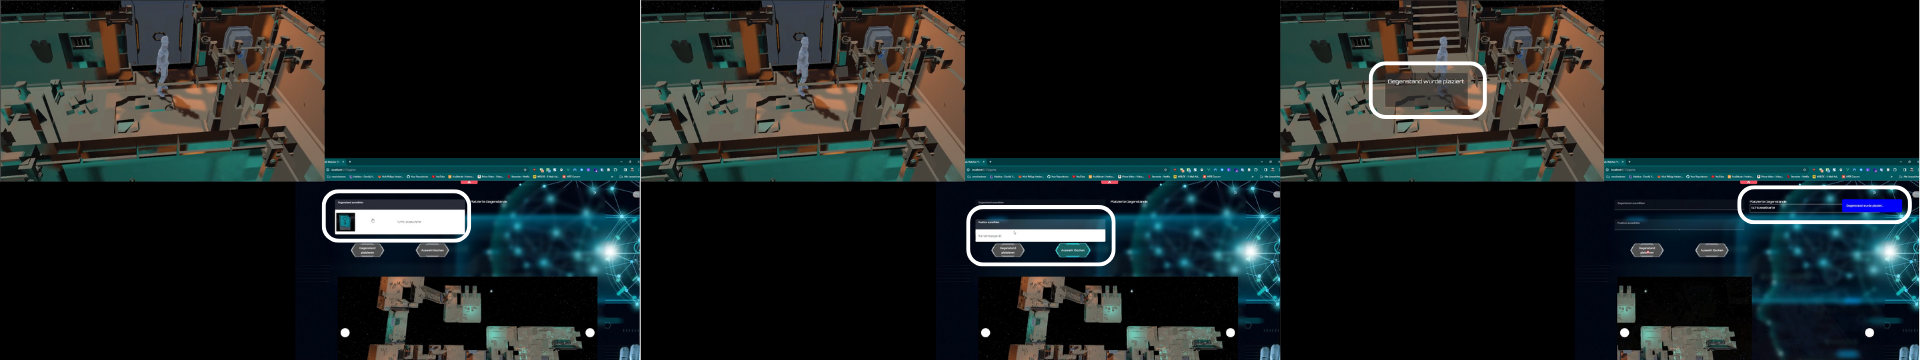
\includegraphics[width=1\linewidth]{content/pictures/HowToSolve.png}
\caption{Vorgang des Lösens von Rätseln (Quelle: eigene Darstellung)}
\label{fig:old-solving-riddle}
\end{figure}

Im früheren Prototyp lag die alleinige Verantwortung für die Lösung der Rätsel beim Watcher. Dieser war dafür zuständig, die richtigen Gegenstände an den jeweils korrekten Zielpositionen zu platzieren. Sobald der Player in der Spielwelt auf eine Absperrung stieß, musste er seine Beobachtungen verbal schildern, um dem Watcher Hinweise darauf zu geben, welche Gegenstände an welchen Positionen benötigt werden.

Der Lösungsprozess verlief wie folgt. Zunächst wählte der Watcher über das Dropdown-Menü für Gegenstände den entsprechenden Gegenstand aus (vgl. Abbildung \ref{fig:old-solving-riddle}, linkes Bild, rechtes Bildelement). Anschließend wählte er eine Zielposition aus einer vordefinierten Liste von Platzierungsoptionen, die in den aktuell aktiven Abschnitten der Spielwelt verfügbar waren (vgl. mittlere Bild, rechts Bildelement). Über den Button \say{Gegenstand platzieren} (linker Button) wird der Gegenstand in die Spielwelt des Players eingefügt.

Nach erfolgreicher Platzierung erhielten sowohl Player als auch Watcher eine visuelle Rückmeldung durch das System (vgl. rechts Bild, beide weiß Umrandeten Elemente). Zusätzlich wurde der neu platzierte Gegenstand automatisch in die Liste der aktuell vorhandenen Gegenstände auf der rechten Seite der Watcher-Anwendung übernommen (rechtes Bild, rechtes Bildelement). 

\subsection{Freischalten von Gegenständen und Positionen}

Sobald ein Rätsel durch das Platzieren der richtigen Gegenstände gelöst wurde, erhielten sowohl der Player als auch der Watcher eine Rückmeldung darüber, dass neue Gegenstände freigeschaltet wurden (vgl. Abbildung \ref{fig:old-unlock-system}, erste Reihe linkes Bild, weiß eingekreist). 

\begin{figure}[ht]
\centering
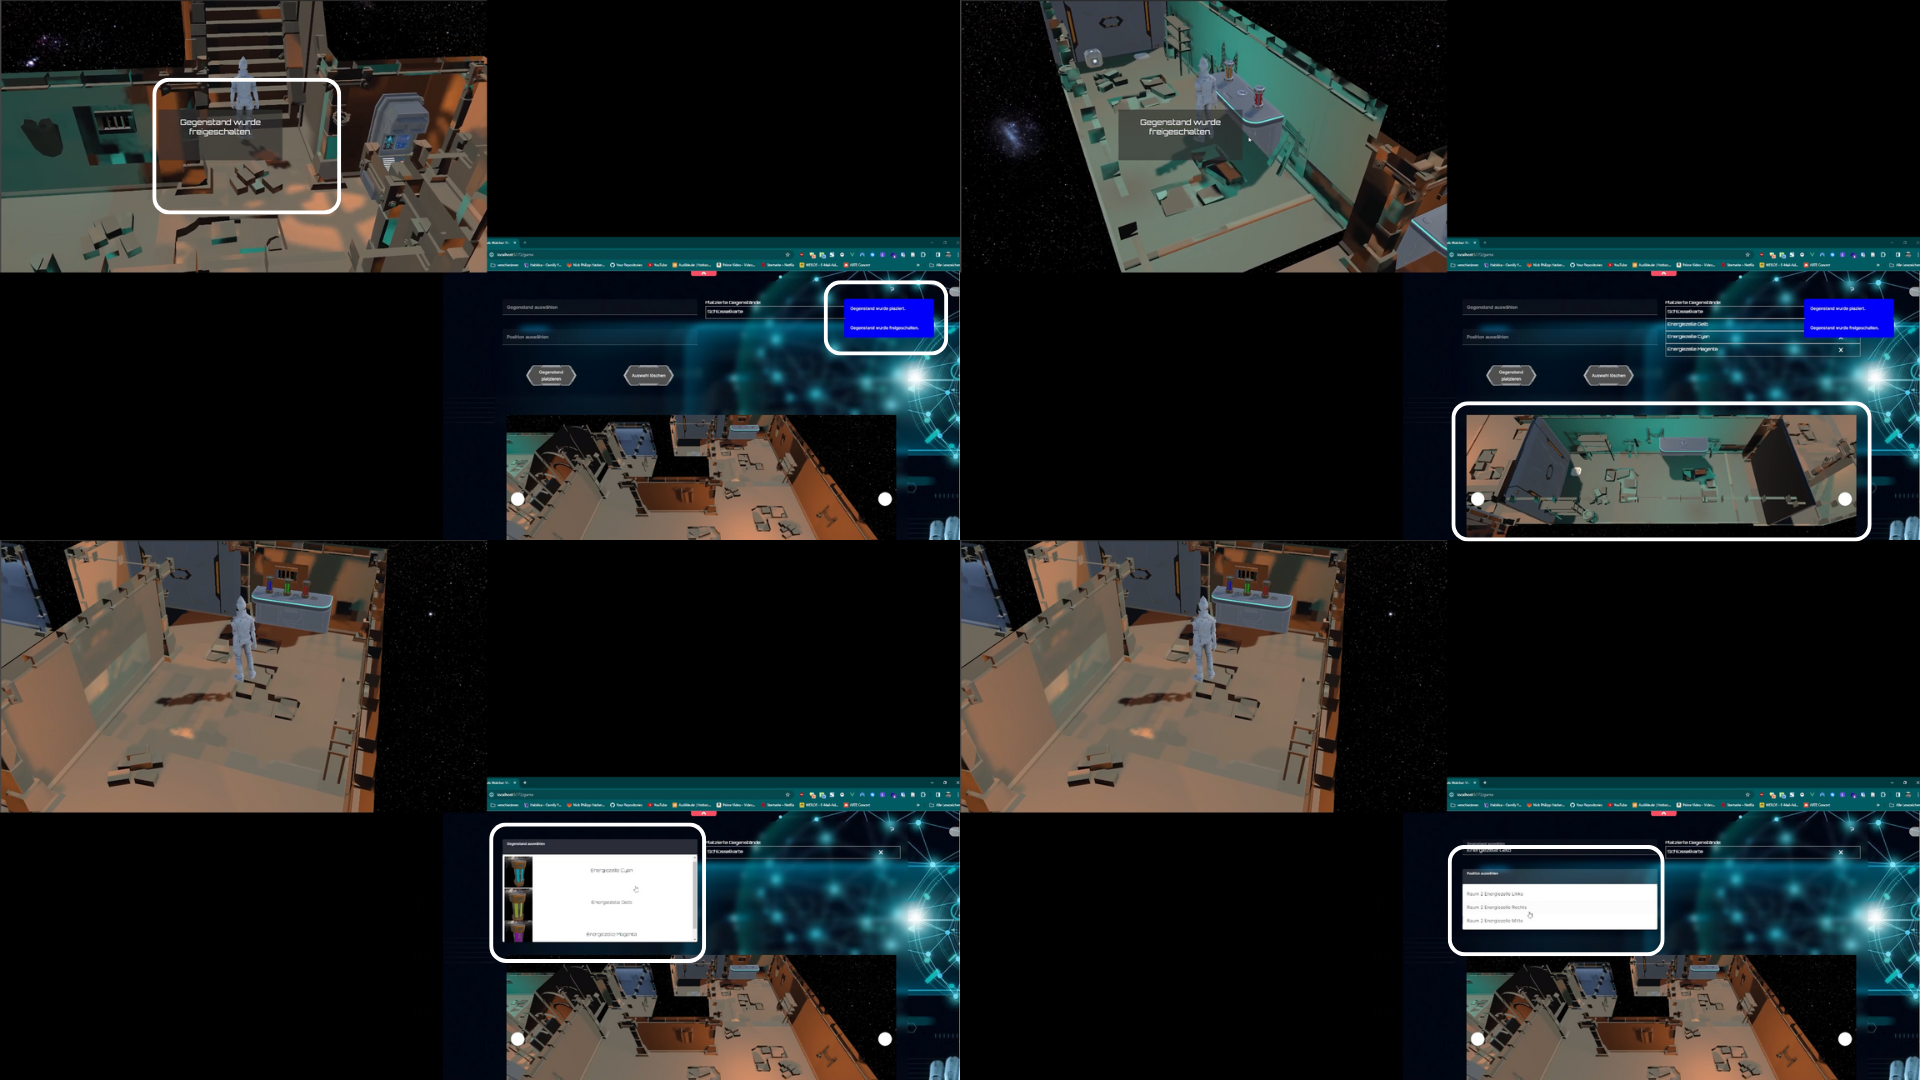
\includegraphics[width=1\linewidth]{content/pictures/UnlockMore.png}
\caption{Freischalten neuer Gegenstände (Quelle: eigene Darstellung)}
\label{fig:old-unlock-system}
\end{figure}

Wenn durch das Lösen des Rätsels ein Hindernis entfernt und ein neuer Bereich der Spielwelt zugänglich gemacht wurde, aktualisierte sich der Bilder-Slider in der Watcher-Anwendung automatisch und wechselte zur aktuell freigeschalteten Ansicht. Der Slider zeigt dem Watcher alle derzeit verfügbaren Abschnitte der Spielwelt  (vgl. Abbildung \ref{fig:old-unlock-system}, erste Reihe, rechtes Bild, weiß umrandet). 

Mit dem Zugang zu neuen Spielabschnitten werden nur nur zusätzliche Gegenstände freigeschaltet, sondern auch weitere vordefinierte Zielpositionen, auf denen diese platziert werden können. Diese neue Optionen erscheinen im Watcher-Interface in den Dropdown-Menüs für Gegenstände und Positionen (vgl. Abbildung \ref{fig:old-unlock-system}, zweiten Reihe, beide Bilder, jeweils weiß umrandet). 

\subsection{Aspekte zum Überarbeiten}

In diesem Kapitel werden jene Aspekte des ursprünglichen Prototyps dargestellt, die in der Umsetzung als unzureichend identifiziert wurden und im Rahmen der Weiterentwicklung im neuen Prototyp überarbeitet werden sollen.

\paragraph{Backfaces}

In den zuvor dargestellten Abbildungen \ref{fig:old-logins} bis \ref{fig:old-unlock-system} ist zu erkennen, dass die Wände der Spielwelt, in der sich der Player befindet (jeweils das linke Bildelement), eine ungewöhnliche und falsche Darstellung aufweisen. Dies liegt daran, dass die verwendeten Raumelemente ursprünglich für eine Kameraperspektive aus dem Inneren des Raums konzipiert wurden. Um eine konkrete Darstellung zu gewährleisten, wäre für diesen Aufbau eine First-Person-Kamera notwendig.

\begin{figure}[ht]
\centering
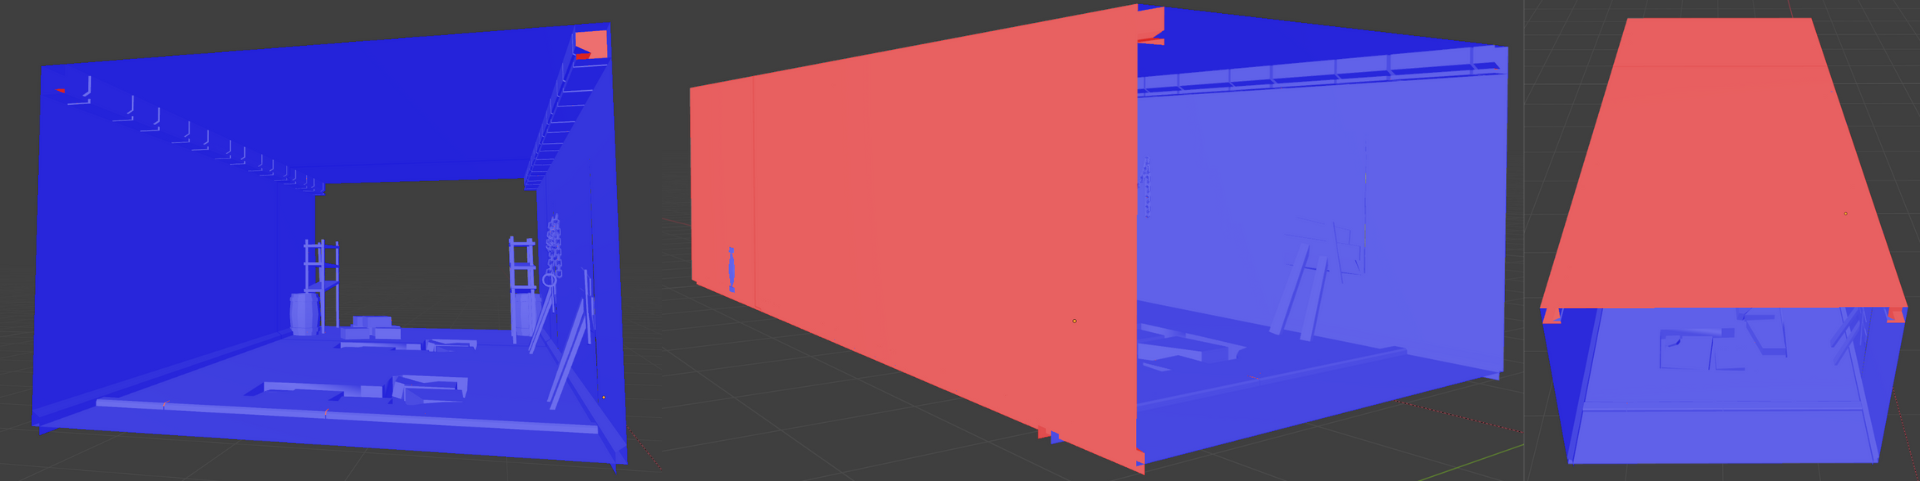
\includegraphics[width=1\linewidth]{content/pictures/Backfaces.png}
\caption{Fehlende Rückwand-Oberflächen in den Raummodellen (Quelle: eigene Darstellung), (Modell von \cite{alasl_autolevel_nodate})}
\label{fig:missing-backfaces}
\end{figure}

Abbildung \ref{fig:missing-backfaces} verdeutlicht, dass Rückseitenflächen bei der aktuellen Modellierung fehlen. Die blauen Flächen kennzeichnen Oberflächen, deren Normalvektoren in Richtung der Kamera zeigen und somit von der Game Engine gerendert werden können. Die roten Flächen hingegen sind Rückseiten, deren Normalvektoren von der Kamera wegzeigen und die daher standardmäßig nicht dargestellt werden.

Zur Behebung dieses Problems bestehen grundsätzlich zwei Lösungsansätze. Entweder wird in der Materialkonfiguration der betroffenen Objekte bidirektionales Rendering aktiviert, oder das Modell wird so angepasst, dass es für jede Betrachtungsrichtung eigene Flächen mit entsprechend ausgerichteten Normalen enthält.

Für die beabsichtige Nutzung in einem Spiel mit Top-Down-Perspektive ist es darüber hinaus erforderlich, die Decken der Räume zu entfernen, da diese aus der gewählten Kameraperspektive nicht sichtbar sind und die Sicht auf relevante Elemente der Spielwelt beeinträchtigen würden.

\paragraph{Steuerung des Avatars}

Im vorangegangenen Prototyp wurde der Gestaltung der Spielsteuerung mittel Touch-Input nur geringe Aufmerksamkeit geschenkt. Die im Projekt zu Beginn eingesetzte Standardsteuerung des verwendeten Unity-Assets von \cite{alasl_autolevel_2022} unterstützte ausschließlich Maus- und Tastatureingaben. Die Fortbewegung innerhalb der Spielwelt erfolgte die Steuerung der Kamera über die Tastatur, ähnlich wie in \ac{RTS}-Spielen, während ein Klick mit der linken Maustaste eine Bewegung des Avatars zur angeklickten Position auslöste.

Eine Steuerung über Touch-Eingaben, etwa an einem Touchscreen-Monitor oder Fernsehgerät, war in der ursprünglichen Implementierung des Beispielprojekts nicht vorgesehen und musste nachträglich ergänzt werden. Das Asset von \cite{alasl_autolevel_2022} nutzt das Cinemachine-Kamerasystem, wodurch einige mausbasierte Kamerasteuerungen bereits vorimplementiert waren (vgl. \citealp{unity_technologies_about_2017}). Eine spezifische Touch-Steuerung hingegen fehlte vollständig.

Die nachträglich hinzugefügte Touch-Eingabe orientierte sich nicht nach etablierten Standards für Touch-Interfaces, wie sie bspw. von \cite{reinhard_augmented_2022} vorgeschlagen werden (vgl. \citealp[S. 64ff]{reinhard_augmented_2022}). Stattdessen wurde eine eigens entwickelte Lösung implementiert, die jedoch nicht denselben Bedienkomfort wie die Maussteuerung bieten konnte.

\paragraph{Interaktion mit der Spielwelt}

Sowohl in der Anwendung des Players als auch in der Watchers bestanden bislang nur sehr eingeschränkte, teils gar keine Interaktionsmöglichkeiten mit der Spielwelt. In der Player-Anwendung beschränkte sich die Interaktion auf das Navigieren innerhalb der Spielumgebung. Die Watcher-Anwendung verfügte hingegen über keinerlei Funktionalitäten im direkten Bezug auf die Spielwelt. Die Interaktion beschränkte sich auf die Menüführung, über die Sitzungsdaten verwaltet werden konnten.

Für den zukünftigen Prototyp ist es daher essenziell, die zentralen Kernfunktionen zu integrieren, die eine vertiefte Interaktion mit der Spielwelt ermöglichen. Nur so kann das interaktive Zusammenspiel zwischen Player und Watcher gewährleistet werden.

\paragraph{Sonstiges Feedback aus den Probandentests}
\begin{figure}[ht]
\centering
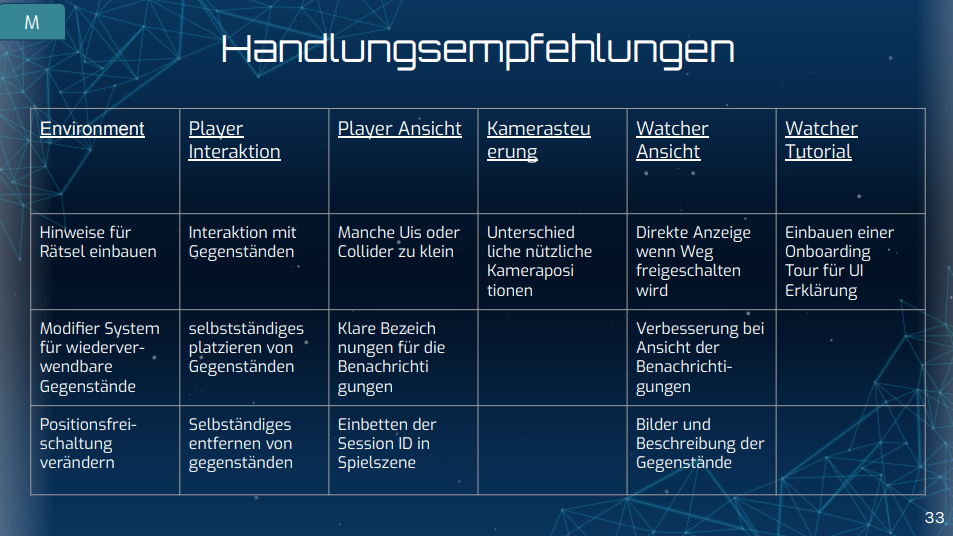
\includegraphics[width=1\linewidth]{content/pictures/Handlungsempfehlungen.PNG}
\caption{Handlungsempfehlungen des alten Prototyps (Quelle: eigene Darstellung aus der Abschlusspräsentation), (ganze Präsentation in Anhang \ref{sec:append_realisation_ausgangslage_presentation}: \nameref{sec:append_realisation_ausgangslage_presentation}, S. 33)}
\label{fig:recommended-action}
\end{figure}

Abbildung \ref{fig:recommended-action} stellt die in der vorangegangenen Arbeit formulierten Handlungsempfehlungen für den ursprünglichen Prototyp dar. Die Bereiche \say{Player Interaktion}, \say{Player Ansicht}, \say{Kamerasteuerung} sowie \say{Watcher Ansicht} wurden in den o. g. Abschnitten bereits thematisiert. Die Punkte \say{Environment} und \say{Watcher Tutorial} blieben bislang unberücksichtigt. Insbesondere das \say{Watcher Tutorial} wurde in der Weiterentwicklung des Prototyps nicht implementiert da der konzeptionelle und technische Aufwand für die Erstellung eines integrierten Tutorials zur Einführung in die \ac{UI}-Elemente als zu hoch eingeschätzt wurde. Ein entsprechendes Tutorials müsste darüber hinaus auch für die Anwendung des Players vorgesehen werden, was den Entwicklungswand weiter erhöht hätte.

Im Folgenden wird der Fokus daher auf das Environment gelegt. Die Handlungsempfehlungen in Abbildung \ref{fig:recommended-action} beziehen sich auf das bestehende System des Prototyps, kassen sich jedoch abstrahieren und auf eine umfassendere Weiterentwicklung übertragen. Eine solche Weiterentwicklung würde neue Möglichkeiten zur Gestellung und Integration von Rätseln innerhalb der Spielwelt eröffnen. So könnten etwas Interaktionspunkte auf der Karte dynamisch und nicht mehr ausschließlich vordefiniert positioniert werden. Ebenso wäre es denkbar bestehende Objekte in ihrer Funktionalität oder Erscheinung zu verändern, um neue Spielmechaniken zu ermöglichen. Diese Potenziale sollten bei einer zukünftigen Neugestaltung des Environments berücksichtigt werden, um die spielerische Tiefe und Varianz zu erhöhen.

\section{Verwendete Technologien}

In der folgenden Auflistung werden sämtliche externen Assets und Packages vorgestellt, die während der Entwicklung des Prototyps zum Einsatz kamen. Einige dieser Assets sind nicht in der Projekt-Registry aufgeführt, da sie zunächst in ein separates Testprojekt importiert, dort bearbeitet und anschließend als angepasste Submodule in das Hauptprojekt integriert wurden.

\subsection{Unity Editor Version 2022.3.45f1}
Der Prototyp wurde mit der 2022.3.45f1 \ac{LTS}-Version umgesetzt, da diese zum Start der Masterarbeit die aktuelle 2022 \ac{LTS}-Version war. Zwischenzeitlich wurde auch die 2023.2.20f1 (vgl. \citealp{noauthor_unity_nodate}) ausprobiert. Da diese allerdings weder eine \ac{LTS}-Version noch zusätzlich im Package der Cinemachine ein Major-Update enthalten war und die Cinemachine einige Probleme mit sich führte, wurde eine stabile 20222-Version gewählt.

\subsection{Blender 4.3.2}
Blender dient als Bearbeitungstool für die 3D-Modelle aus den hinzugenommenen Unity Assets. Die aktuelle Version zu Projektstart war die 4.3.2 Version- welche über den gesamten Bearbeitungszeitraum verwendet wurde. Außerdem bietet Unity einen Blender Direktimport an, wodurch keine \ac{FBX} oder \ac{OBJ} Dateien aus den Blenderdateien exportiert und in Unity importiert werden mussten.

\subsection{NuGetForUnity 4.1.1}
NuGetForUnity ist ein für Unity entwickelter NuGet-Client (vgl. \citealp{noauthor_nuget_nodate}) über den zusätzliche funktionale Pakete für Unity installiert werden kann (vgl. \citealp{mccarthy_glitchenzonugetforunity_2025}). Er war nötig, um ein nicht über Unity erworbenes Package in Unity nutzen zu können. Die aktuelle Version zum Bearbeitungsstart war die 4.1.1 Version, welche bis zum Ende genutzt wurde.

\subsection{Newtonsoft.Json 13.03}
Das erste Package, welches über NuGetForUnity installiert wurde ist Newtonsoft.Json, durch welches über den WebSocket übertragene JSON-Daten leicht deserialisiert und serialisiert werden können (vgl. \citealp{newtonsoft_jsonnet_nodate}). Die aktuelle Version im NuGet-Paketverwaltungstool war die 13.03.

\subsection{WebSocketSharp-netstandard 1.0.1}
Derzeit gibt es einige Netzwerk-Integrationen für Unity, bspw. Mirror (vgl. \citealp{noauthor_mirror_nodate}) oder Netcode for GameObjects (vgl. \citealp{noauthor_about_2025}). Durch die beiden Packages wäre jedoch die Netzwerk-Topologie starrer und die Entwicklung nach eigener Vorstellung wäre ebenfalls eingeschränkter. Daher wurde über NuGetForUnity das WebSocketSharp-netstandard Paket installiert, welches eine direkte Kommunikation mit einem WebSocket-Server ermöglicht (vgl. \citealp{pingman_tools_pingmantoolswebsocket-sharp_2025}), da bislang existierende Integration mit Unity nicht mehr unterstützt werden. Die derzeit installierte und zum Projektstart installierbare Version ist die 1.0.1.

\subsection{AI Navigation 1.1.5}
Da sich der Avatar des Players innerhalb der Spielwelt per Touch-Click auf den Bildschirm an die angeklickte Stelle bewegen soll, muss ein \ac{AI}-Agent eingebaut werden, der das Avatar Spielobjekt an die gewünschte Stelle bewegt. In Unity kann dafür das NavMesh System verwendet werden, welches ein Pathfinding-System implementiert, wodurch ein automatisiertes Bewegen eines Agents durch eine Zielposition integriert werden kann. Das Paket in Unity heißt \ac{AI}-Navigation. Die aktuelle Version zum Start des Projekts ist die 1.1.5.

\subsection{Cinemachine 2.10.1}
Die Cinemachine wurde in der Entwicklung des Prototyps bei beiden Anwendungen als unterstützendes Element für die Kamerasteuerung verwendet. Durch die Cinemachine können virtuelle Kameras genutzt werden, durch welche verschiedene Ansichten in der Spielwelt erstellt werden können. Außerdem unterstützt sie bei der Kameraführung ein verfolgtes Objekt, wie dem Avatar des Players. Zudem es ist durch sie möglich, auf einfache weise eine Zoom-Funktion einzubauen. Die aktuelle Version für die 2022-Unity Version ist die 2.10.1, welche über den gesamten Verlauf der Arbeit verwendet wurde.

\subsection{Universal RP 14.0.11}
Für die Entwicklung einer Anwendung für Mobile Endgeräte oder die für Windows-Geräte kann die \ac{URP} verwendet werden. Außerdem ist die \ac{URP} mit ARFoundation kompatibel, wodurch die Wahl auf die \ac{URP} und nicht die Built-In Render Pipeline fiel. Die zum Start und über den Verlauf der Arbeit genutzte Version ist die 14.0.11.

\subsection{Unity UI 1.0.0 und TextMeshPro 3.0.9}
Für die Entwicklung der \ac{UI}-Elemente der Anwendungen wurden die Pakete Unity \ac{UI} und TextMeshPro in ihren zum Start des Projekt aktuellen Versionen verwendet. Unity \ac{UI} ist dabei das Standard-Paket für die Entwicklung von User-Interfaces. TextMeshPro erweitert die Standard \ac{UI}-Elemente von Unity \ac{UI} um weitere Komponenten, welche für die Entwicklung des \ac{UI}s verwendet wurden.

\subsection{Input System 1.7.0}
Seit der 2022er-Unity Version wird empfohlen das neue Input System von Unity zu verwenden. Das alte Input System ist standardisiert in jedem Unity Projekt enthalten und wird durch das neue, das Paket Input System überschrieben. Es ermöglicht über ein eigenes Menü verschiedene Input-Möglichkeiten zu konfigurieren und innerhalb der Scripte zu verwenden.

\subsection{FBX Exporter 4.2.1}
Manche Meshes der verwendeten Unity-Assets waren nicht im Binary-\ac{FBX}-Format importiert,  wodurch sie über den \ac{FBX} Exporter zu einer Binary-\ac{FBX} Datei exportiert werden konnten. Außerdem kam es vor, dass manche Assets keine grundlegenden Meshes enthielten, wodurch die enthaltenen Prefabs zu \ac{FBX}-Dateien exportiert werden mussten. Die aktuelle Version des Exporters zum Start des Projekts war die 4.2.1.

\subsection{AR Foundation 5.1.6}
Für die Entwicklung von \ac{AR}-Anwendungen in Unity gibt es verschiedene Möglichkeiten. Die gängigsten Auswahlmöglichkeiten sind hierbei Vuforia (vgl. \cite{noauthor_home_nodate}) oder das Unity interne Paket AR Foundation (vgl. \cite{noauthor_ar_nodate}). Die AR Foundation ermöglicht im Vergleich zu Vuforia auf mehreren Arten das Tracking und Platzieren von virtuellen Gegenständen. Darum fiel die Wahl auf AR Foundation. Außerdem ist die AR Foundation leichter in die Versionierung in Git einzubinden. Hierbei gab es in vergangenen Projekten durch zu große Konfigurations-Dateien von Vuforia Probleme.

\subsection{Google ARCore XR Plugin 5.1.6}
In Abhängigkeit zum Paket AR Foundation wurde auch das Google ARCore Modul installiert, welches wichtig für mobiles \ac{AR} auf Android Smartphones ist. Es bietet eine Schnittstelle zwischen den Android eigenen Modulen auf dem Smartphone und der Unity Anwendung.

\subsection{Unity Assets}
Da durch den begrenzten Bearbeitungszeitraum keine Zeit blieb in großen Maßen eigene \ac{3D}-Objekte zu modellieren, wurde dafür auf bestehende und zum größten Teil kostenlose Assets zurückgegriffen, welche alle über den Unity Asset Store erworben werden konnten. Die enthaltenen Objekte wurden jedoch in einer großen Nacharbeitung an die eigenen Anforderungen angepasst und in die eigenen Submodule importiert.
\begin{itemize}  
    \item Astronaut - Free Model By Quaternius von \cite{quaternius_astronaut_2022}
    \item low poly WD | 3D Props 1.1 \cite{squid_low_2023}
    \item Adventure Game Environment Pack | URP | 3D Sci-Fi 1.0 \cite{unity_technologies_adventure_2023}
    \item Adventure - Sample Game | Tutorials 3.0 \cite{unity_technologies_adventure_2024}
    \item Bedroom / Interior - Low Poly assets | 3D Interior 1.1.6 \cite{fries_and_seagull_bedroom_2025}
    \item Big Furniture Pack | 3D Furniture 1.3 \cite{vertex_studio_big_2027}
    \item Chair pack - 3D Low Poly Office Furniture - Created with FastMesh Asset | 3D Furniture 1.0 \cite{fast_mesh_chair_2024}
    \item Fantasy Cemetery \& Necropolis Pack Lite: 3D Assets for RPG and Adventure Games | 3D Fantasy 1.2 \cite{emaceart_fantasy_2022}
    \item Free Wood Door Pack | 3D Interior 1.0 \cite{biostart_free_2024}
    \item Kitchen Appliance - Low Poly | 3D Electronics 1.02 \cite{alstra_infinite_kitchen_2021}
    \item Lowpoly Dungeon Assets | 3D Dungeons 1.0 \cite{kunniki_lowpoly_2018}
    \item Low Poly Dungeon Generator | 3D Dungeons 1.0 \cite{mysticforge_low_2025}
    \item Low Poly Dungeons Lite | 3D Dungeons 1.11 \cite{justcreate_low_2024}
    \item Low Poly Simple Medieval Props | 3D Props 1.0 \cite{justcreate_low_2023}
    \item LowPoly Server Room Props | 3D Environments 1.0 \cite{ipoly3d_lowpoly_2021}
    \item Melon's Low Poly Office | 3D Interior 1.1.1 \cite{mistyczny_arbuz_melons_2022}
    \item Office Pack - Free | 3D Interior 1.02 \cite{nappin_office_2024}
    \item Ultimate Low Poly Dungeon | 3D Dungeons 2.0 \cite{broken_vector_ultimate_2022}
\end{itemize}

\subsection{Node Version 20.18.1}
Für den WebSocket-Server wurde eine Laufzeitumgebung benötigt, welche die zum Zeitpunkt des zugrunde liegenden Projekts die Node Version 20.18.1 war. Da das Teilprojekt des WebSocket-Servers aus dem vorangegangenen Projekts wiederverwendet werden konnte, wurde die Node Version beibehalten.

\subsection{Express.js Webserver 5.1.0}
Express.js ist eine Webserver Erweiterung von Node.js Servern, durch diese spezifische \ac{URL}-Endpunkte erstellt werden können. Über diese \ac{URL}-Endpunkte lassen sich Funktionen realisieren, die der Server haben soll. Zusätzlich benötigt das Package WS einen Express.js Server um über diesen einen WebSocket-Server zu starten. 

\subsection{WS 8.18.2}
WS ist das \ac{NPM}-Paket, über welches der WebSocket-Server implementiert werden kann. Das Paket ist innerhalb eines Express.js Server einfach zu verwenden und ermöglicht es Nachrichten zu empfangen und zu senden. Außerdem können empfangene Nachrichten in einem internen Mechanismus weitergereicht werden, wodurch für verschiedene Nachrichten Arten verschiedene Klassen gebaut werden konnten (vgl. \citealp{websockets_websocketsws_2025}).

\subsection{Docker}
Docker ist eine Open-Source-Plattform über die Container erstellt, bereitgestellt, ausgeführt, aktualisiert und verwaltet werden können. Container sind standardisierte, ausführbare Komponenten, die den Code von einzelnen Anwendungen mit den Betriebssystembibliotheken und Abhängigkeiten kombinieren (vgl. \citealp{noauthor_was_2024}). Docker wurde aus dem Grund eines möglichen späteren Deployments des WebSocket-Server verwendet, da aus dem erstellen Express.js Server ein Docker-Image erstellt werden könnte, und so die öffentliche Bereitstellung vereinfacht worden wäre. Außerdem können über die Docker Engine weitere Images importiert werden, welche lokal auf dem Gerät laufen und so eine Unabhängigkeit zum Internetzugang bestehen kann.

\subsection{MongoDB - Docker Image}
MongoDB bietet über das eigene Atlas System einen Online-Zugriff auf definierten Datenbanken an. Diese sind nur über das Internet erreichbar. Eine Anfrage an die Online-Datenbank könnte Latenzzeiten enthalten, wodurch der Prozess gestört werdem würde. Daher wurde ein Docker Image für eine MongoDB Umgebung verwendet. Dieses Image ist aus der Docker Community und für jeden frei zugänglich (vgl. \citealp{noauthor_mongo_nodate}). Diese läuft auf dem Rechner, auf dem Docker läuft und ist innerhalb dieses Rechners über den definierten Port erreichbar.

\subsection{node-mongodb-native NPM-Paket}
Um innerhalb des Express.js Servers eine Verbindungen zur MongoDB Datenbank aufbauen zu können, existiert eine Library, die Zugänge und weitere Funktionen im Bezug auf MongoDB bereitstellt. Das \ac{NPM}-Paket \say{node-mongodb-native} wurde für diesen Zweck verwendet (vgl. \citealp{mongodb_mongodbnode-mongodb-native_2025}).


\subsection{User Interface Inspirationen}
Für die bisherig Implementierten \ac{UI}-Elemente wurden bestehende Bilder oder Icons nachgezeichnet und als Vorlage für eine Weiterentwicklung des \ac{UI}s eingebaut. Im folgenden werden die Quellen aufgezählt.

\begin{itemize}
    \item Vorlage für SciFi \ac{UI}s von \cite{pchvector_free_nodate}
    \item Vorlage für Low-Poly Feder von \cite{masud_download_nodate}
    \item Vorlage für die Rucksack Icon in Anhang \ref{sec:append_realisation_vorlage_rucksack}
    \item Vorlage für das Positions zurücksetzen Icon \cite{noauthor_chatgpt_nodate-3}
    \item Vorlage für das Hinweis Icon \cite{noauthor_chatgpt_nodate-2}
    \item Vorlage für Interaktions Icon \cite{noauthor_chatgpt_nodate-1}
    \item Vorlage für die Bücher Icons \cite{noauthor_chatgpt_nodate}
    \item Vorlage für die Handzeichnung in Anhang \ref{sec:append_realisation_vorlage_handzeichnung}
\end{itemize}

\section{Aufbau des Prototyps}

Der neue Prototyp ist, analog zum vorhergehenden Projekt, in drei separate Einzelprojekte untergegliedert: Die Anwendungen für Player, Watcher und Server. Diese drei Komponenten wurden entsprechend der \ac{MVC}-Architektur strukturiert. Die Server-Anwendung ais dem vorherigen Projekt konnte in diesem Zusammenhang übernommen und funktional erweitert werden. Ihre Architektur ist spezifisch auf das Zusammenspiel innerhalb dieses Aufbaus ausgerichtet. Die Wahl dieser Struktur basierte ursprünglich darauf, dass im vorherigen Projekt jedes Gruppenmitglied einen eigenständigen Implementierungsteil bearbeiten und abgeben musste. Die klare Trennung der Zuständigkeit innerhalb der \ac{MVC}-Architektur unterstütze dabei.

\subsection{Player-Anwendung}

Die Player-Anwendung stellt eine der beiden \say{Views} innerhalb des entworfenen Systems dar. Sie bildet primär die Spielwelt ab, in der sich der Avatar des Players während der Laufzeit bewegt. Der Aufbau der Spielwelt basiert auf einem Submodul des Projekts, das zentrale Basismodelle bereitstellt. Diese Modelle werden im jeweiligen Projektkontext als \say{Prefab Variants} angepasst. Auf diese Weise kann sichergestellt werden, dass die zugrunde liegende Struktur der Spielwelt sowohl in der Player- als auch in der Watcher-Anwendung konsistent bleibt, während spezifische Unterschiede gezielt integriert werden können.

\paragraph{Steuerung der Anwendung}

Ein zentrales Element der Player-Anwendung ist die Steuerung des Avatars. Im ursprünglichen Projekt war vorgesehen, dass die Anwendung auf einem Touchmonitor, etwa einem kleinen Display oder einem Smartboard, bedient werden kann. \cite{reinhard_augmented_2022} weist darauf hin, dass Multitouch-Anwendungen typischerweise Interaktionen wie Pan (Verschiebung auf der X- und Y-Achse), Zoom, Yaw (Rotation um die vertikale Achsel mittel Fingerbewegung) sowie Pitch (Veränderung des Neigungswinkels) unterstützen (vgl. \citealp[S. 66ff]{reinhard_augmented_2022}).

Für die konkrete Umsetzung bedeutet dies, dass zunächst festgelegt werden muss, wie die Kamera auf die Spielszene sowie auf den Avatar ausgerichtet ist und gesteuert wird. Unity stellt mit dem Cinemachine-Paket ein flexibles und leistungsfähiges System zur Kamerasteuerung bereit. Die sog. \say{Free-Look Camera} ermöglicht dabei eine freie Kameraführung um ein definiertes Zielobjekt. Voraussetzung hierfür ist die Angabe eines \say{Follow}- und eines \say{LookAt}-Objekts, um die Kamera automatisch an das Ziel anzugleichen.

Die Cinemachine-Komponenten sind standardmäßig für Maus-Inputs optimiert. Um die Kamera jedoch auch auf Touch-Eingaben zu übertragen, müssen die von Reinhard beschriebenen Multitouch-Gesten implementiert werden. Die Pan-Geste, also das horizontale oder vertikale Verschieben eines Fingers über den Bildschirm, wird genutzt, um die Kamera rotierend um den Avatar zu bewegen. Diese ersetzt die Mausbewegung, mit der in der Standardeinstellung um das LookAt-Objekt rotiert wird.

Ergänzend wird die Zoom-Geste, bei der zweu Finger zueinander oder voneinander wegbewegt werden, verwendet, um die Kamera entlang der Z-Achse näher an den Avatar heranzuführen oder sich von ihm zu entfernen. Damit wird das in der Cinemachine integrierte Zoom-Verhalten für die Maussteuerung auf Touch-Eingaben übertragen.

Für die Fortbewegung des Avatars reicht eine einfache Single-Touch-Geste aus, bei der eine Position in der Spielwelt angetippt wird. Der Avatar soll sich anschließend zu dieser Position bewegen. Hierfür kommt das in Unity integrierte \say{NavMesh-Agent}-System zum Einsatz. Dieses basiert auf einem Pathfinding-Algorithmus der es dem Agent ermöglicht, autonom ein Ziel innerhalb eines zuvor definierten Navigationsbereichs (\say{NavMesh Surface}) anzusteuern. Die Zielposition wird per Touch übermittelt, woraufhin sich der Avatar eigenständig dorthin bewegt. Dank der Verbindung zur Cinemachine-Komponente folgt die Kamera dem Avatar während seiner Bewegung automatisch.

\paragraph{Questsystem}\label{sec:quest-system}

Da die Rätsel und Hindernisse nicht willkürlich ohne System in der Spielwelt platziert wurden, wurde ein modulares System entwickelt, das den systematischen Aufbau und die Kombination unterschiedlicher Rätselkomponenten ermöglicht.

\begin{figure}[ht]
\centering
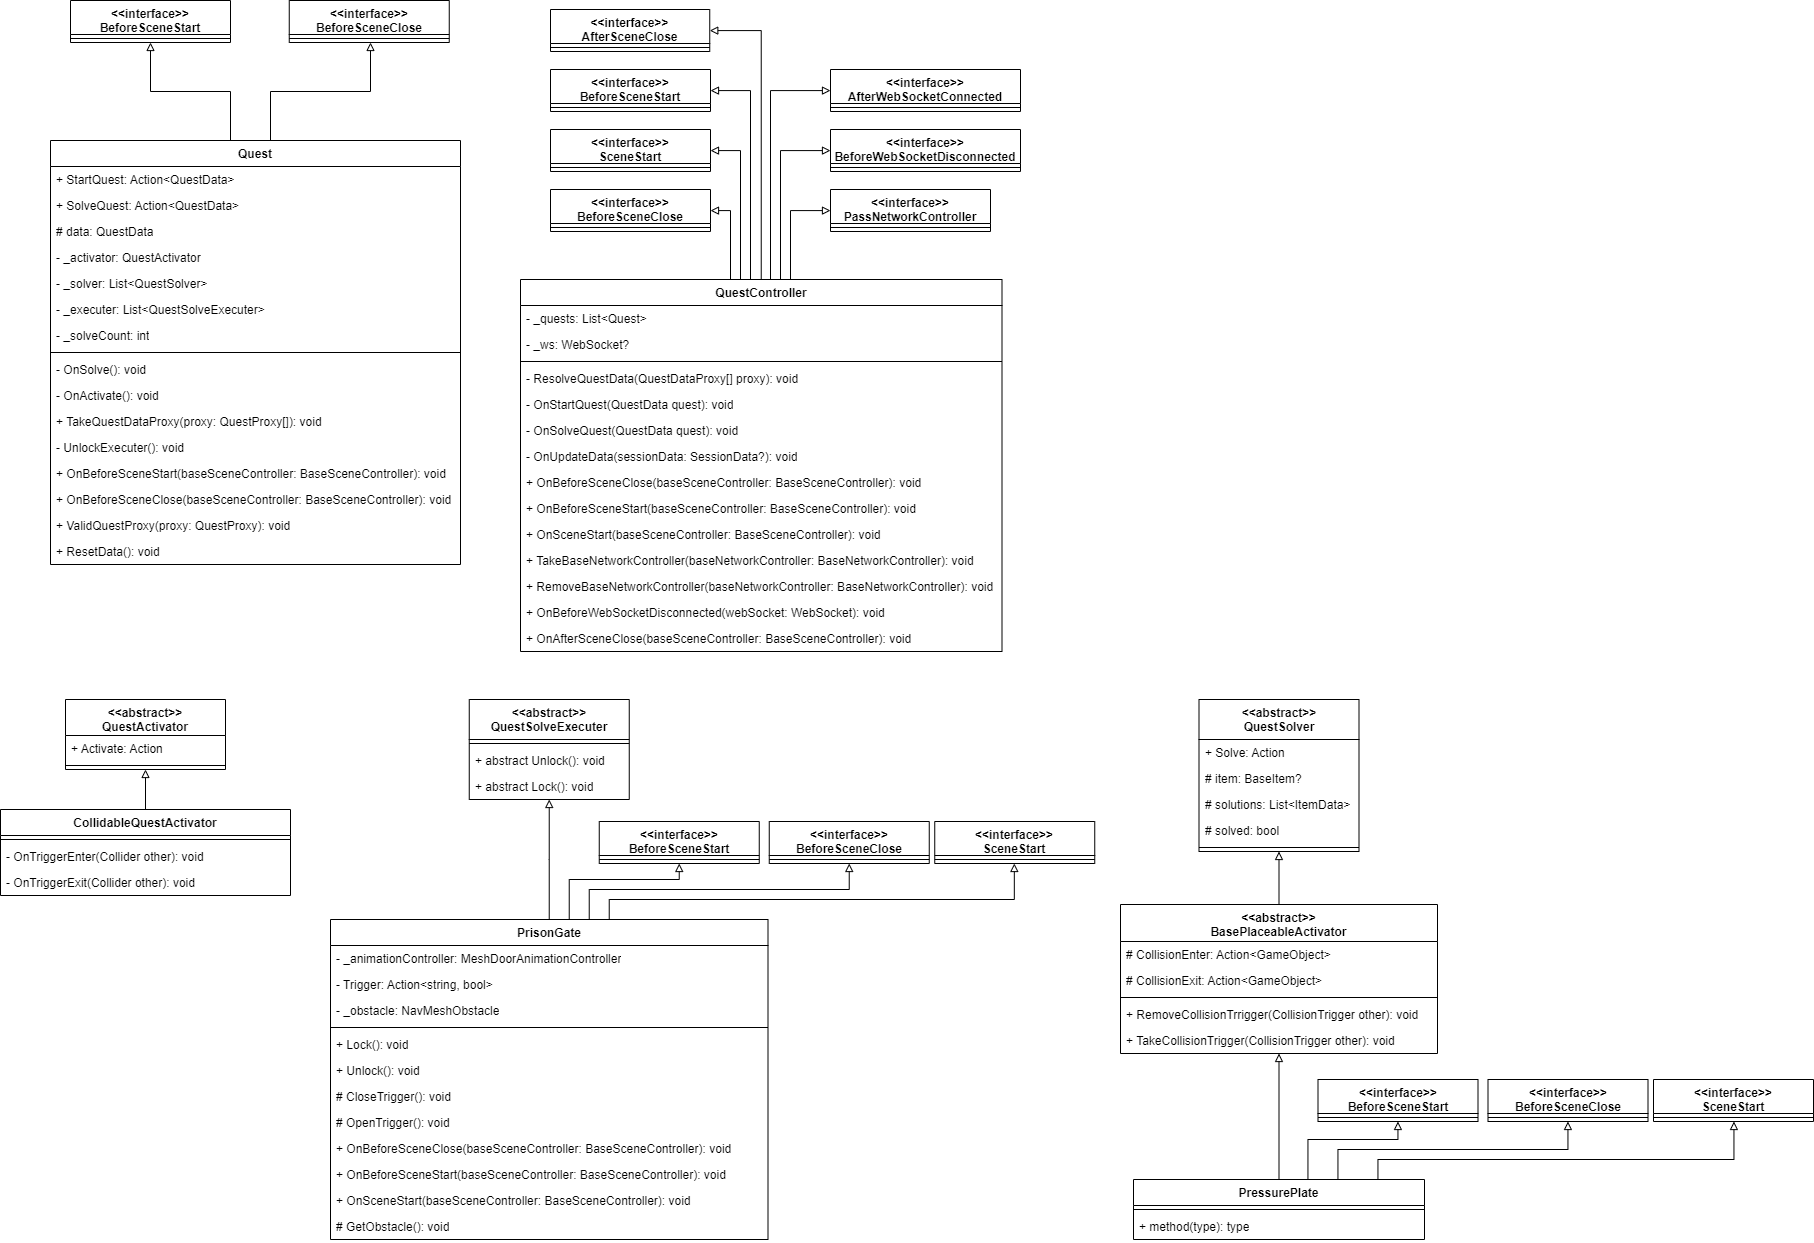
\includegraphics[width=1\linewidth]{content/pictures/QuestSystem.drawio.png}
\caption{UML-Diagramm zum Questsystem (Quelle: eigene Darstellung), (vollständig in Anhang \ref{sec:append_realisation_uml_quest})}
\label{fig:quest-system-uml}
\end{figure}

Abbildung \ref{fig:quest-system-uml} zeigt, das entwickelte Questsystem, das zur strukturierten Einbettung von Rätsel in die Spielwelt dient. Die einzelnen Rätsel wurden in Anlehnung an \ac{RPG}-Spiele als Quests bezeichnet. Das System wurde modular konzipiert, sodass es sowohl in der Player- als auch in der Watcher-Anwendung integriert werden kann. Die folgenden Ausführungen gelten daher für beide Rollen gleichermaßen.

Zentrale Instanz des Systems ist der QuestController, der als überwachende Einheit fungiert. Er verwaltet Referenzen auf alle in der Szene existierenden Quests, empfängt Rückmeldungen über gelöste Quests vom Server und leitet diese an die entsprechenden Quests weiter. Gleichzeitig ist er für die Übermittlung neuer oder gelöster Quests an den Server verantwortlich. Wird bspw. eine Quest aktiviert, etwa durch das Freischalten eines neuen Raums, sorgt der QuestController dafür, dass diese zur Liste der aktiven bzw. gelösten Quests hinzugefügt wird.

Jede Quest selbst stellt eine einzelne Herausforderung dar und ist mit einer eindeutigen ID, einem Namen sowie einem Lösungsstatus ausgestattet. Sie überprüft selbstständig, ob sie gelöst wurde und informiert in diesem Fall den QuestController. Dazu besitzt sie Referenzen auf mehrere QuestSolver, also logische Einheiten, die eine Bedingung zur Lösung erfüllen müssen. Im Beispiel aus Abbildung \ref{fig:quest-system-uml} handelt es sich um eine Druckplatte mit Platzierungsfunktionalität, die dann aktiv wird, wenn ein passender Gegenstand korrekt platziert wurde. Sobald alle zugehörigen QuestSolver erfolgreich ausgelöst wurden, gilt die Quest als gelöst.

Vor der Lösung muss eine Quests jedoch zunächst aktiviert werden. Diese Funktion übernehmen sog. QuestActivator, auf die jede Quest ebenfalls Referenzen besitzt. Erst wenn alle Aktivatoren ausgelöst wurden, wird die Quest aktiv und kann gelöst werden. Im gezeigten Beispiel kommt ein CollidableQuestActivator zum Einsatz, der dann ausgelöst wird, wenn sich der Avatar des Players innerhalb eines definierten Colliders aufhält.

Sobald eine Quest erfolgreich abgeschlossen wurde, werden alle ihr zugewiesenen QuestSolveExecuter aktiviert. Diese Komponenten führen Aktionen aus, etwa das Öffnen einer Tür durch einen Animator, wie im Beispiel der Gefängnistür dargestellt.

\paragraph{Pathsystem}\label{sec:path-system}

Wie das Questsystem wurde auch das Pathsystem modular konzipiert, um eine Wiederverwendung sowohl in der Player- als auch der Watcher-Anwendung zu ermöglichen. Dieses System ist insbesondere deshalb von zentraler Bedeutung, weil im Verlauf des Spiels neue Wege und Räume zugänglich gemacht werden, deren Freischaltung eng mit dem Fortschritt im Rätselsystem verknüpft ist.

\begin{figure}[ht]
\centering
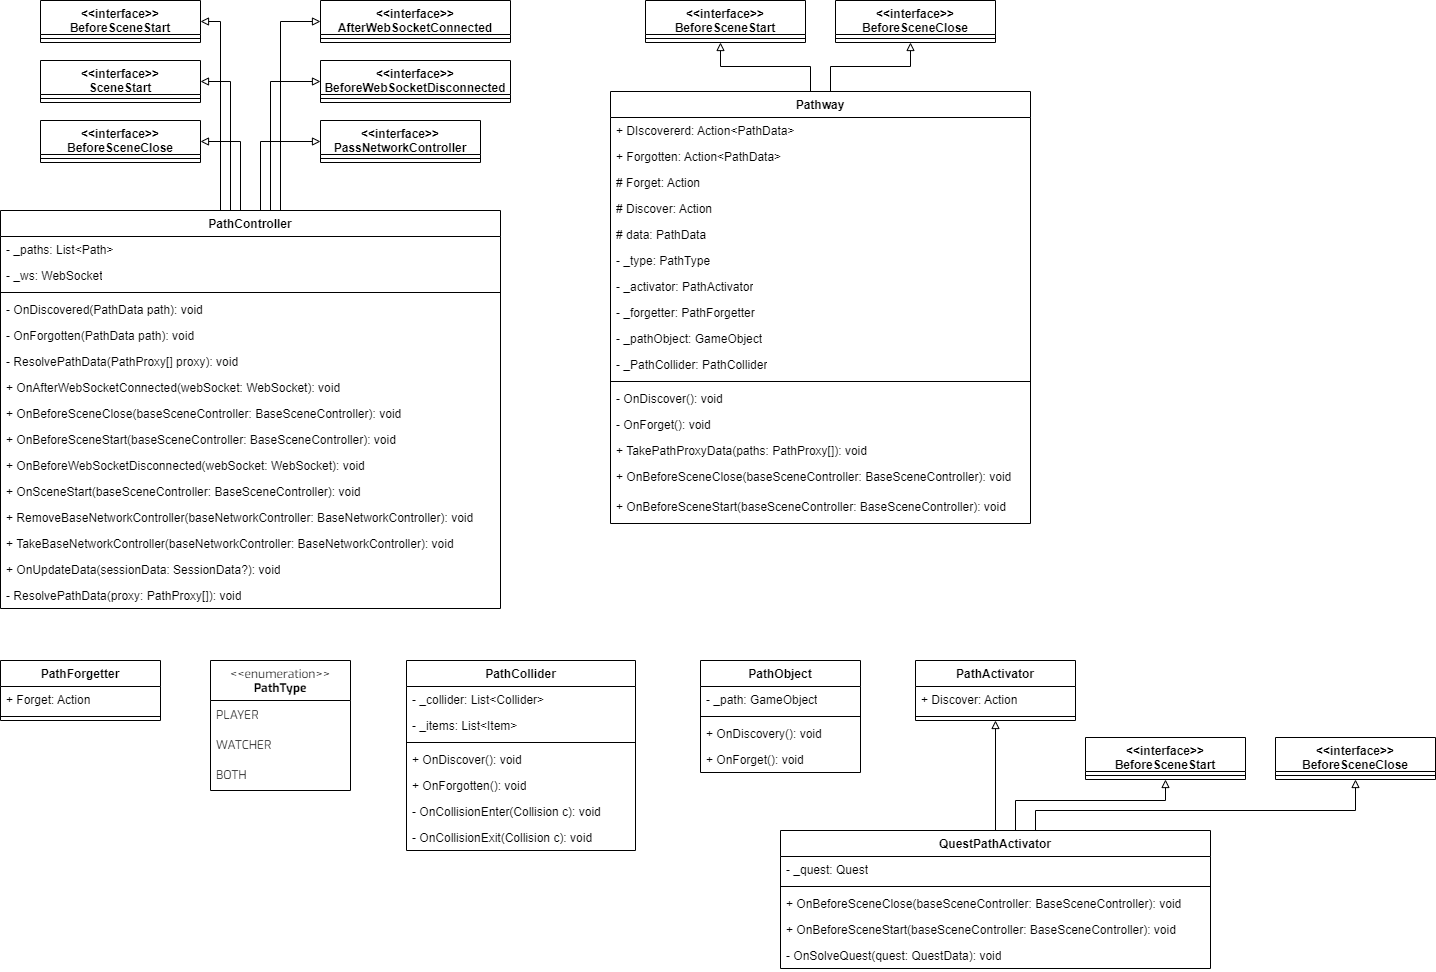
\includegraphics[width=1\linewidth]{content/pictures/PathSystem.drawio.png}
\caption{UML-Diagramm zum Pathsystem (Quelle: eigene Darstellung), (vollständig in Anhang \ref{sec:append_realisation_uml_path})}
\label{fig:path-system-uml}
\end{figure}

Abbildung \ref{fig:path-system-uml} zeigt das entworfene modulare Pathsystem, das in beiden Anwendungen eingebunden ist. Das zentrale Steuerelement stellt die Klasse PathController dar, welche, analog zum QuestController, für die Kommunikation mit dem Server verantwortlich ist. Sie empfängt und sendet Pathdaten und verwaltet sämtliche in der Spielszene konfigurierten Wege (Pathways).

Jeder Pathway verwaltet eine Reihe von Komponenten. Sog. PathActivator, die für die Freischaltung eines Weges zuständig sind und optional PathForgetter, welche bereits geöffnete Wege bei Bedarf wieder deaktivieren können. Darüber hinaus besitzt ein Pathway Referenzen auf die zugehörigen Objekte in der Spielwelt, ein sichtbares Wegobjekt (PathObject) sowie auf Kollisionsbereiche (PathCollider). Letztere spielen insbesondere bei der physischen Blockierung von noch nicht zugänglichen Bereichen eine Rolle.

Da im konzipierten Tutorial-Szenario keine bereits geöffneten Wege deaktiviert werden, wurde auf eine Implementierung konkreter PathForgetter verzichtet. Die Klasse QuestPathActivator aus dem in Abbildung \ref{fig:path-system-uml} dargestellten Beispiel übernimmt die Aufgabe, nach dem erfolgreichen Abschluss einer bestimmten Quest den zugehörigen Pathway zu aktivieren.

Wird ein Pathway aktiviert, so wird das entsprechende \ac{3D}-Objekt (PathObject) in der Szene sichtbar geschaltet und die zugehörigen PathCollider deaktiviert, sodass der neue Bereich für den Player zugänglich wird. Auf die genaue Funktionsweise der PathCollider und deren Bedeutung im Gesamtsystem wird im späteren Kapitel \ref{sec:difficulties-placement} detailliert eingegangen.

\paragraph{User-Interfaces}

\begin{figure}[ht]
\centering
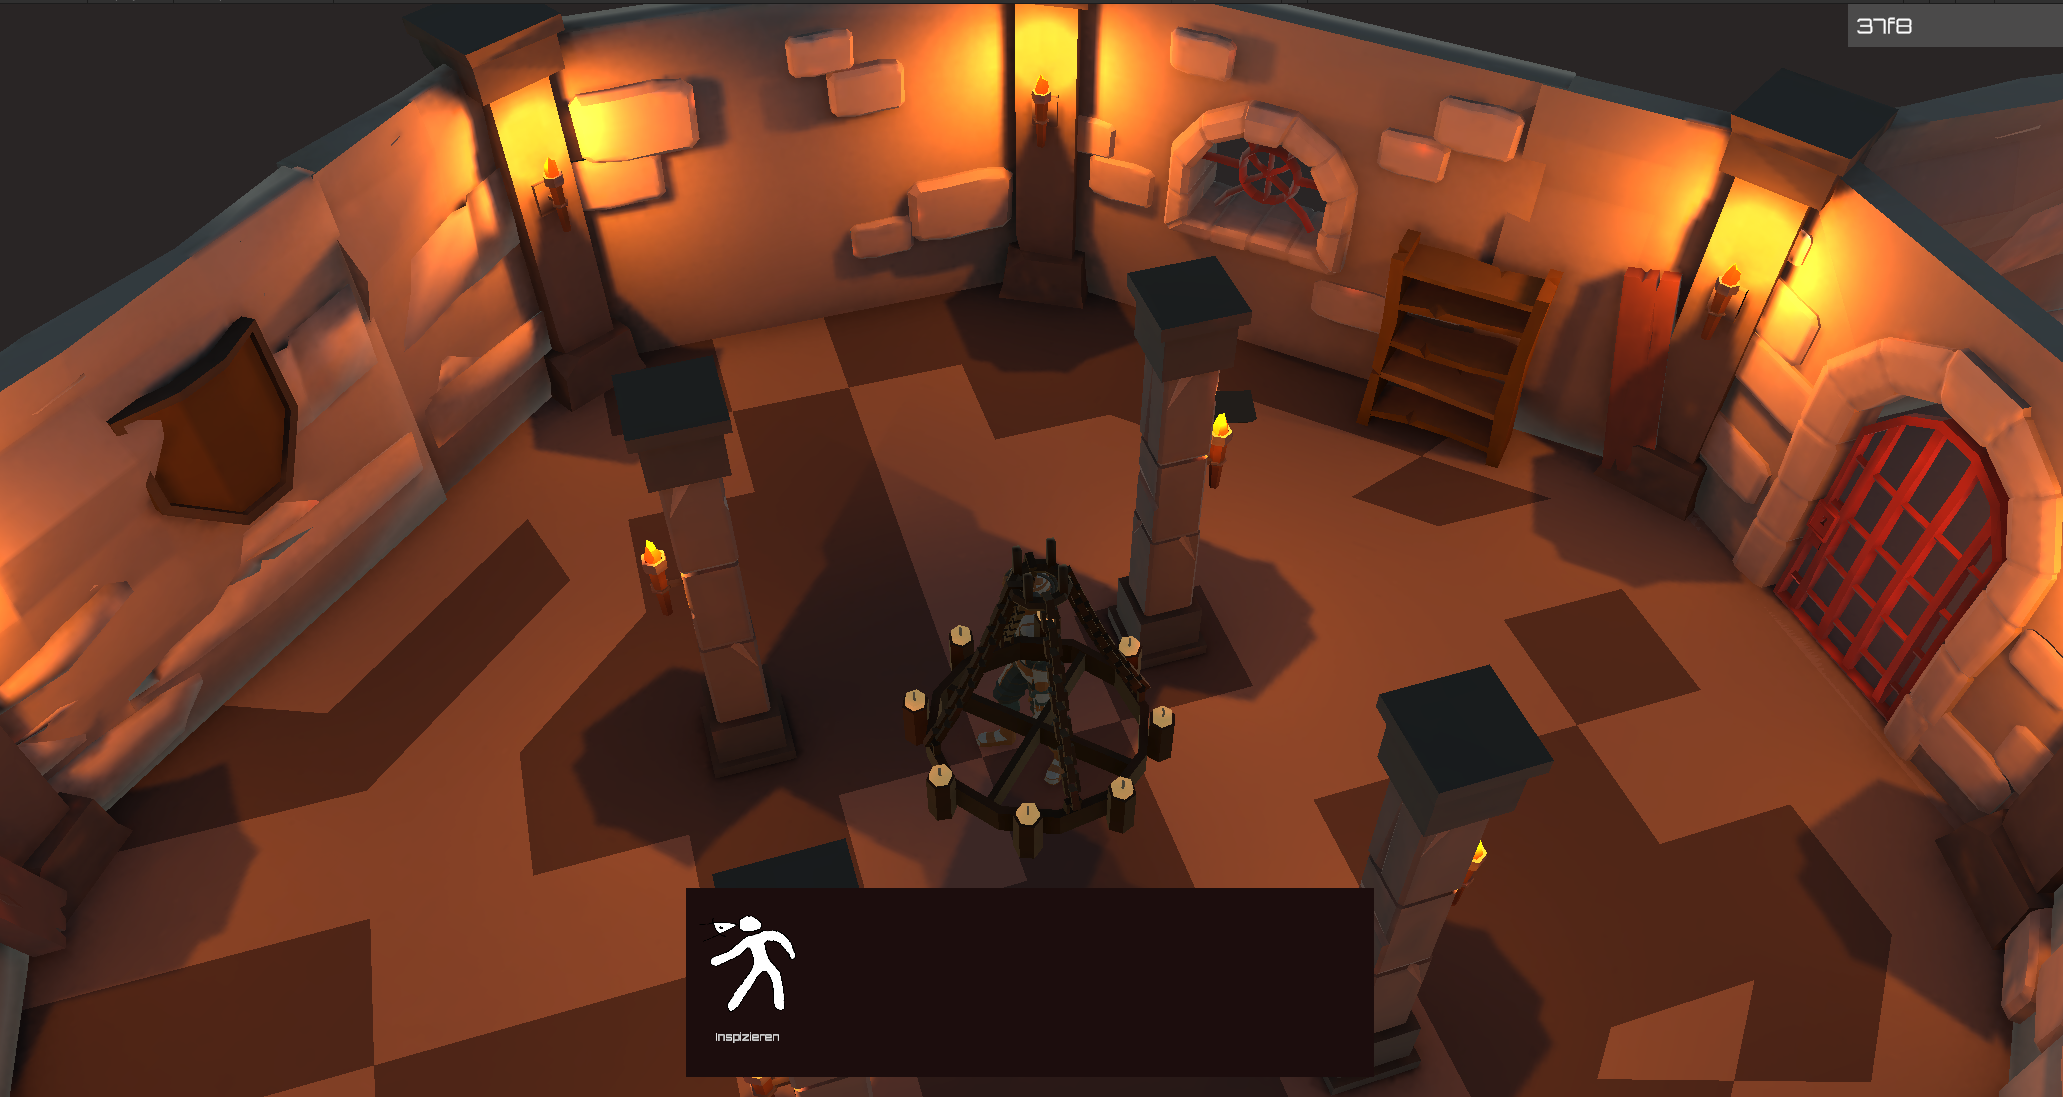
\includegraphics[width=1\linewidth]{content/pictures/UI.PNG}
\caption{UI des Players (Quelle: eigene Darstellung)}
\label{fig:player-ui}
\end{figure}

Abbildung \ref{fig:player-ui} zeigt die Ansicht, die der Player in der Spielwelt hat. Unten in der Mitte wird die Interaktionsleiste angezeigt, über welche der Player Interaktionen mit der Spielwelt ausführen kann. Anhand des gezeigten Bildes kann er derzeit nur in die First-Person-Sicht wechseln. Sobald er an einen interaktiven Gegenstand kommt, erscheint in der Leiste seine entsprechenden Interaktionsfunktionen. Dieses Konzept ist an Spiele wie \say{Diablo 4} oder \say{Baldurs Gate 3} angelehnt, bei denen über eine ähnliche Aktionsleiste Fähigkeiten und Angriffe ausgeführt werden können  (vgl. \citealp{blizzard_entertainment_diablo_2023,larian_studios_baldurs_2023}).

\subsection{Watcher-Anwendung}

Die Watcher-Anwendung stellt, ebenso wie die Player-Anwendung, eine der beiden \say{Views} innerhalb der umgesetzten \ac{MVC}-Architektur dar. Sie umfasst die grundlegende Spielwelt aus der Perspektive des Watchers und bildet zugleich die Grundlage für dessen Interaktionsmöglichkeiten mit der Umgebung.

Analog zur Player-Anwendung basiert auch die visuelle Darstellung in der Watcher-Anwendung auf den Basisobjekten der Spielwelt, die mittels sog. Prefab Variants darstellungsspezifisch angepasst wurden. Auf diese Weise wird eine konsistente Gestaltung der Umgebung sichergestellt, wobei sich für die jeweilige Perspektive relevanten Unterschiede manifestieren.

Ein wesentlicher Unterschied zur Player.Anwendung besteht in der Existenz zweier unterschiedlicher Betriebsmodi. Der Watcher kann entweder mittels einer \ac{AR}-Integration oder über eine \ac{3D}-Ansicht auf die Spielwelt zugreifen. Während die \ac{AR}-Variante für den späteren produktiven Einsatz konzipiert ist, wurde die \ac{3D}-Integration primär für Entwicklungs- und Testzwecke realisiert. Sie ermöglicht es, den aktuellen Entwicklungsstand direkt im Unity-Editor zu überprüfen, ohne dass die Anwendung jeweils auf ein Smartphone übertragen und oder ausgeführt werden muss.

\paragraph{Steuerung der Anwendung}

Wie bereits in der Player-Anwendung spielt auch in der Watcher-Anwendung die Kamerasteuerung eine zentrale Rolle. Allerdings muss sie hier differenzierter betrachtet werden, da sich die Anforderungen in den beiden Modi, \ac{AR} und \ac{3D}, deutlich unterscheiden.

In der \ac{AR}-Variante übernimmt das Endgerät die Kamerasteuerung automatisch über die Sensorsysteme. Eine manuelle Steuerung den Watcher ist daher nicht erforderlich. Für die Interaktion mir der Anwendung genügt eine einfache Single-Touch-Eingabe, etwa zur Platzierung von Gegenständen. Wie \cite{reinhard_augmented_2022} zeigt, sind solche minimalistischen Eingabekonzepte typisch für \ac{AR}-Anwendungen auf Mobilgeräten (vgl. \citealp[S. 66ff]{reinhard_augmented_2022}).

 Gegensatz dazu erfordert die \ac{3D}-Variante der Anwendung eine explizite Kamerasteuerung, ähnlich wie in der Player-Anwendung. In diesem Kontext sind zunächst grundsätzliche Überlegungen zum zugrunde liegenden Kamerakonzept notwendig. Mobile Spiele nutzen unterschiedliche Steuerungsarten. Einige verzichten gänzlich auf eine freie Kamerabewegung, andere folgen einem Spieler-Avatar, während wieder andere eine vollständige Kontrolle über die Kamera ermöglichen.

 Für die \ac{3D}-Variante wurde bewusst auf die Implementierung eines Joystick-basierten \ac{HUD}-Overlays verzichtet, da dieses der intuitiven Touchsteuerung-Nutzung widerspricht und Interaktionsmöglichkeiten unnötig einschränkt. Stattdessen orientierte sich die Umsetzung an Spielen, die auf Touch-Gesten basieren, etwa \say{Die Sims Mobile} oder \say{Outlanders} (vgl. \citealp{arts_sims_2017, pomelo_games_outlanders_2019}). Diese nutzen ein Kamerasystem, wie es aus klassischen Strategiespielen, wie der \say{Anno}-Reihe, bekannt ist, eine, sog. \ac{RTS}-Kamera, bei der ein unsichtbares LookAt und Follow Objekt durch Nutzereingaben verschoben wird, dem die Kamera folgt (vgl. \citealp{noauthor_ubisoft_nodate}). 

Auch in der Watcher-Anwendung wurde dieser \ac{RTS}-Ansatz umgesetzt. Dabei wird die Kamera durch folgende Touch-Gesten gesteuert.
Der Single-Touch für das Platzieren und Entfernen von Gegenständen in der Spielwelt, die Yaw-Geste für die horizontale Rotation der Kameraansicht zur Veränderung der Blickrichtung, die Zoom-Geste für die Annäherung und Entfernung zur Spielwelt und die Pan-Geste zur Bewegung der Kamera innerhalb der Spielwelt.

Die Pitch-Geste wurde bislang nicht implementiert, da für sie in der aktuellen Fassung der Anwendung kein konkreter Anwendungsfall identifiziert wurde.

\paragraph{Aufbau des Nutzerflows}
Da die Hauptaufgabe des Watchers das Verwalten und Platzieren von Gegenständen ist, muss zunächst analysiert werden, wie ein für die Anforderungen an die Anwendungen passender Nutzerfluss konzipiert und umgesetzt werden kann.

Das Spiel \say{Outlanders} (vgl. \cite{pomelo_games_outlanders_2019}) passte in seinem Spielaufbau und seiner Führung durch die Menüs zu der Anforderung der Watcher Anwendung, bei der sich der Spieler zunächst frei durch die Spielwelt bewegen (entweder als \ac{AR}-Kamera oder über das RTS-Kamerasystem), über ein Menü Gegenstände platzieren oder dem Player schicken kann.

In \say{Outlanders} muss der Spieler als Anführer der gemeinen Bevölkerung eine Stadt errichten. Dies kann er über ein Hauptmenü initiieren, welches sich in seiner Menüleiste befindet.

\begin{figure}[ht]
\centering
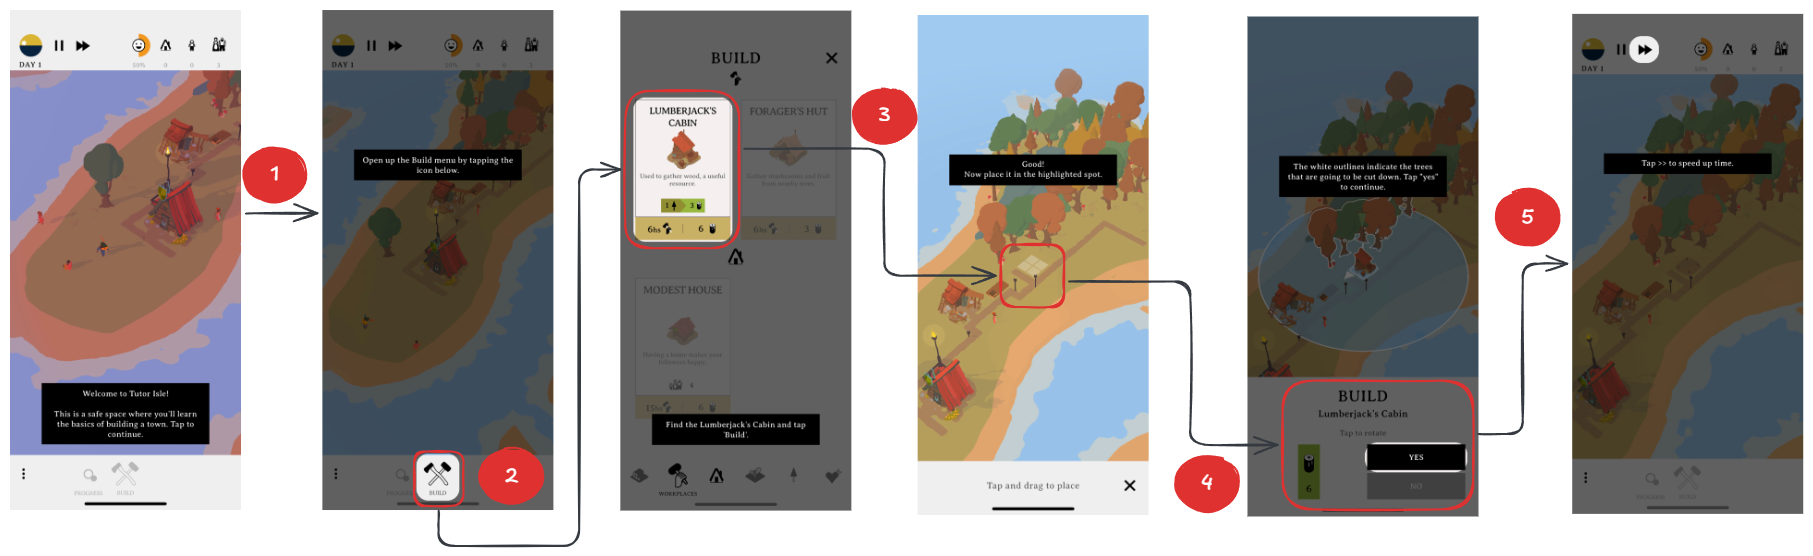
\includegraphics[width=1\linewidth]{content/pictures/Nutzerflow.png}
\caption{Nutzerfluss beim Gebäudebau in Outlanders (Screenshots von \cite{coates_game_nodate}), (Quelle: eigene Darstellung), (groß in Anhang \ref{})}
\label{fig:userflow-outlanders-build}
\end{figure}

Zunächst kann der Spieler sich frei durch die Spielwelt bewegen (1). Sobald der Spieler ein Gebäude für seine Bevölkerung bauen möchte, muss er in der Menüleiste am unteren Ende des Bildschirms auf den Reiter \say{Build} klicken (2). Darauffolgend öffnet sich ein Overlay-Menü, welches das Baumenü darstellt. In ihm kann der Spieler zwischen verschiedenen Kategorien von Gebäuden und anderen Bauelementen wechseln. Klickt er auf ein gewünschtes Gebäude, schließt sich das Menü und er muss nun in der Spielwelt auf die Stelle klicken, wohin das ausgewählte Gebäude platziert werden soll (3). Wurde eine Position gewählt, öffnet sich ein weiteres Menü, welches nur über die Hälfte des Bildschirmes geht, in welchem der Spieler bestätigen muss, dass das Gebäude an diese Stelle platziert werden soll (4). Nachdem er bestätigt hat, wird das Gebäude platziert und das Bestätigungs-Menü geschlossen. Der Spieler kann nun wieder frei durch die Spielwelt navigieren (5).

Nicht nur der Nutzerfluss des Baumenüs wurde übernommen, sondern auch die Eindrücke des \ac{UI}s haben einen sehr starken Einfluss auf die ersten \ac{UI}s der Anwendung.

\begin{figure}[ht]
\centering
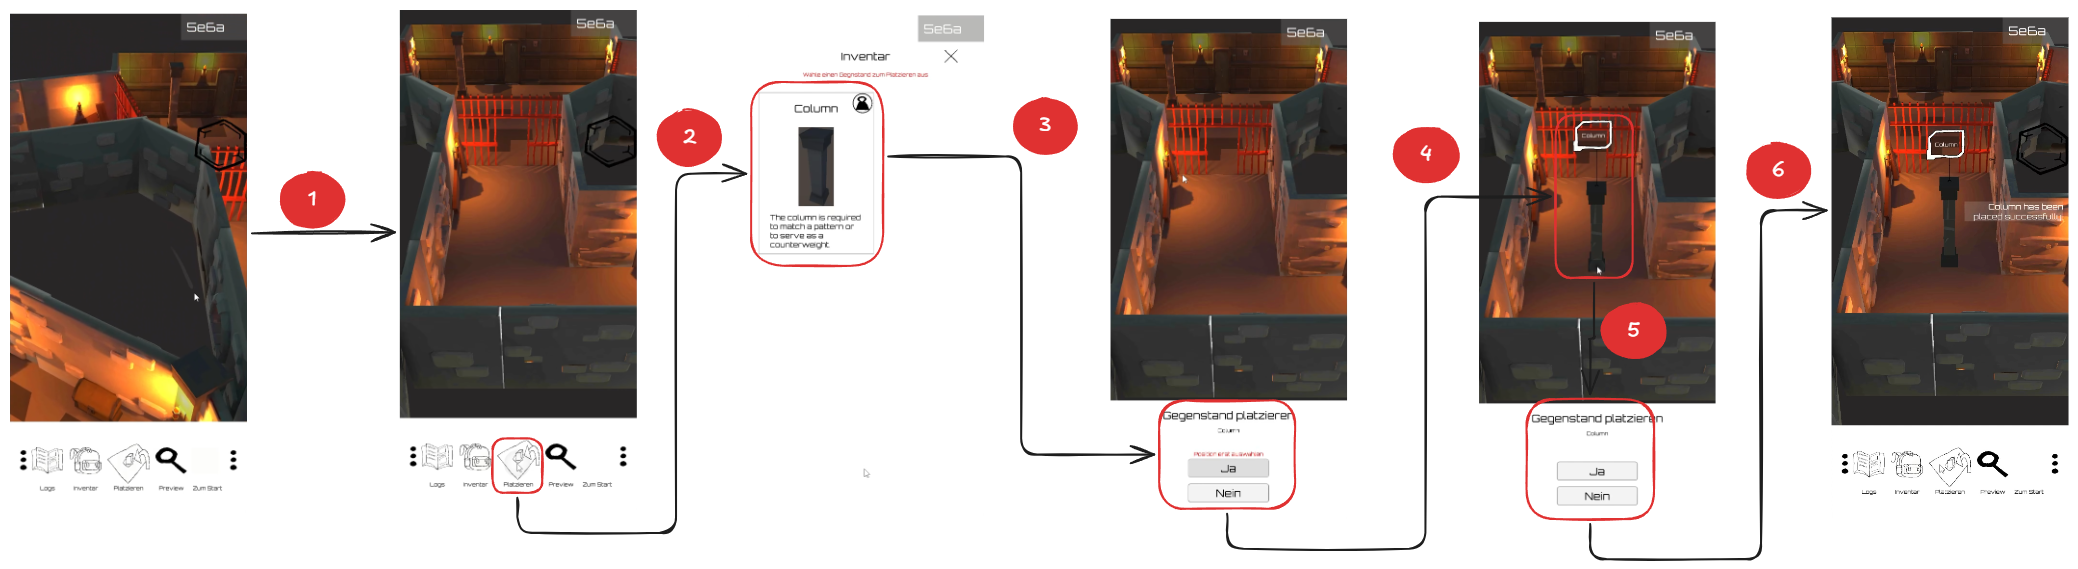
\includegraphics[width=1\linewidth]{content/pictures/PlacementFlow.png}
\caption{Nutzerfluss des Platzierens eines Gegenstandes (Quelle: eigene Darstellung), (groß in Anhang \ref{})}
\label{fig:userflow-placement-cm}
\end{figure}

Abbildung \ref{fig:userflow-placement-cm} zeigt den Nutzerfluss, den ein Spieler durchgeht, wenn er einen Gegenstand platzieren will. Er ähnelt sehr stark dem aus Outlanders. Zunächst kann sich der Watcher frei durch die Spielwelt bewegen (1). Nun muss er an einer bestimmten Stelle einen Gegenstand platzieren. Er klickt auf das Platzieren Menü und ein Overlay-Menü öffnet sich (2). Über das Menü kann er nun einen Gegenstand zum Platzieren auswählen (3). Sobald ein Gegenstand ausgewählt wurde, öffnet sich ein Menü, welches einen kleineren Teil des Bildschirms abdeckt und den Watcher auffordert eine Position zu wählen (3). Nachdem eine Position gewählt wurde, sieht der Watcher das zukünftig platzierte Objekt auf der gewählten Position (4). Über das noch aktive Menü kann der Nutzer nun die Platzierung des Gegenstandes bestätigen (5). Wurde die Wahl bestätigt, so steht nun an der gewählten Stelle der gewünschte Gegenstand (6). 

\begin{figure}[ht]
\centering
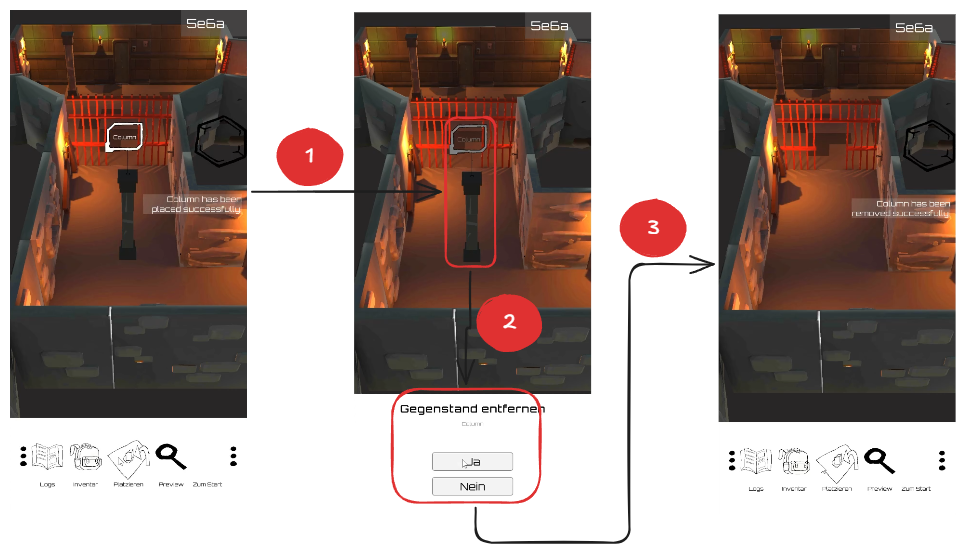
\includegraphics[width=1\linewidth]{content/pictures/RemovePlacementFlow.png}
\caption{Nutzerfluss des Entfernens eines Gegenstandes (Quelle: eigene Darstellung), (groß in Anhang \ref{})}
\label{fig:userflow-removement-cm}
\end{figure}

Abbildung \ref{fig:userflow-removement-cm} zeigt den Nutzerfluss, den ein Watcher durchläuft, sobald er einen platzierten Gegenstand wieder entfernen möchte. Zunächst kann sich hier der Watcher frei durch die Welt bewegen. Er muss nun aber einen Gegenstand entfernen, damit er ihn an einer anderen Stelle wieder platzieren kann. Er klickt nun auf den in der Spielwelt platzierten Gegenstand (1). Das Tooltip des ausgewählten Gegenstands verändert sich farblich, um dem Spieler zu zeigen, welcher Gegenstand ausgewählt wurde. Außerdem öffnet sich ein kleines Menü am unteren Ende des Bildschirmes, über welches der Watcher das Entfernen des Gegenstandes bestätigen kann (2). Nachdem das Entfernen bestätigt wurde, kann sich der Watcher wieder frei durch die Welt bewegen (3).

\begin{figure}[ht]
\centering
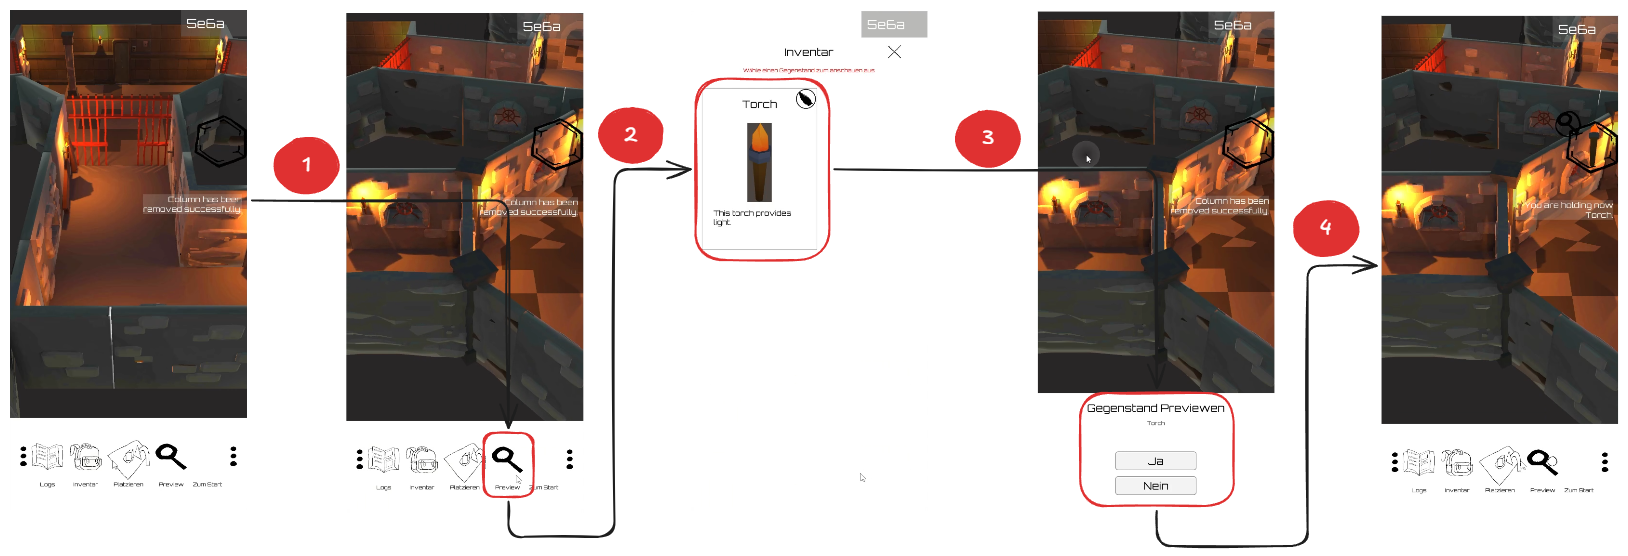
\includegraphics[width=1\linewidth]{content/pictures/PreviewFlow.png}
\caption{Nutzerfluss des Previewen eines Gegenstandes (Quelle: eigene Darstellung), (groß in Anhang \ref{})}
\label{fig:userflow-preview-cm}
\end{figure}

Neben dem Platzieren eines Gegenstandes ist auch das Schicken eines Gegenstandes an den Player eine wichtige Aufgabe des Watchers. Der vorangegangene Nutzerfluss aus der Vorlage von Outlanders und der bereits erfolgreichen Integration in den Nutzerfluss des Platzierens, wurde nun auch für das Previewen von Gegenständen eingesetzt (vgl. Abbildung \ref{fig:userflow-preview-cm}).

Nachdem sich der Watcher frei durch die Spielwelt bewegen konnte, muss er nun dem Player einen bestimmten Gegenstand schicken (1). Über das \say{Preview}-Menü, rechts neben dem \say{Platzieren}-Menü, kann der Watcher das Schicken initialisieren. Klickt er auf das Menü, öffnet sich auch hier eine Galerie, die über den ganzen Bildschirm geöffnet wird. Hier kann der Spieler nun den gewünschten Gegenstand auswählen (2). Sobald ein Gegenstand ausgewählt wurde, öffnet sich ein Bestätigungsmenü, bei dem er die Auswahl bestätigen muss (3). Nachdem die Auswahl bestätigt wurde, kann sich der Watcher auch hier wieder frei durch die Welt bewegen. Er sieht an der rechten, halb hohen Seite, den Gegenstand, den der Player nun trägt (4).

\begin{figure}[ht]
\centering
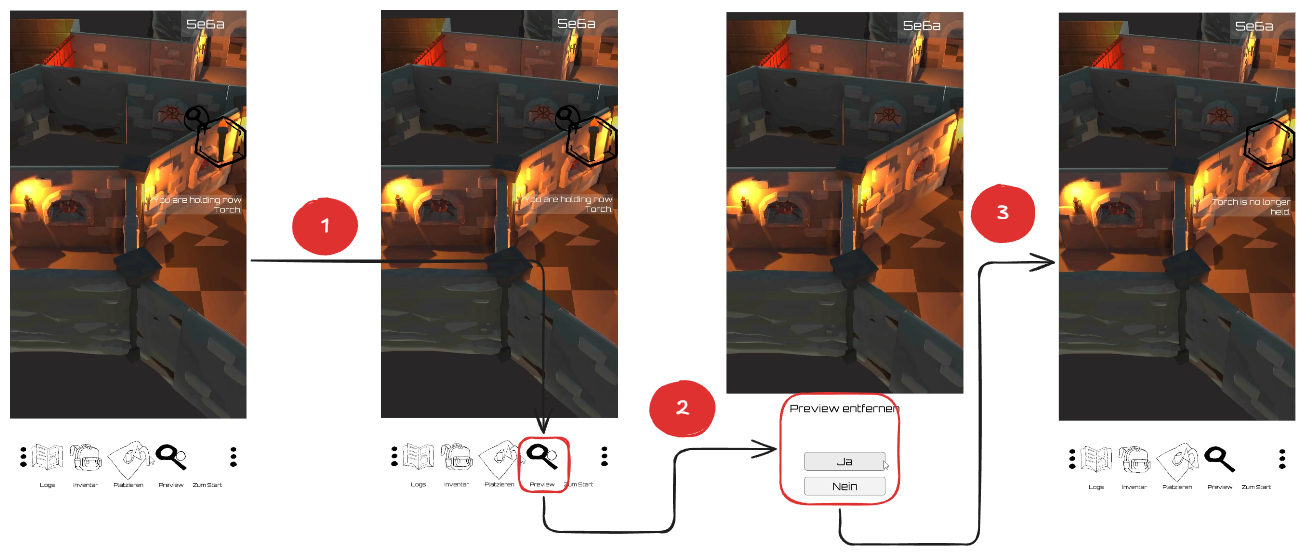
\includegraphics[width=1\linewidth]{content/pictures/RemovePreviewFlow.png}
\caption{Nutzerfluss des Entfernens der Preview eines Gegenstandes (Quelle: eigene Darstellung), (groß in Anhang \ref{})}
\label{fig:userflow-remove-preview-cm}
\end{figure}

Abbildung \ref{fig:userflow-remove-preview-cm} zeigt den Nutzerfluss des entsprechenden Entfernens der Preview eines Gegenstandes. Zunächst kann sich der Watcher noch frei durch die Welt bewegen. Sobald er einen Hinweis bekommt, dass er einen Gegenstand wieder entfernen soll, kann er wie beim Schicken eines Gegenstandes auf das \say{Preview}-Menü klicken (1). Nachdem er darauf geklickt hat, öffnet sich nicht wie beim ersten Mal ein Menü, sondern direkt das Überprüfungs-Menü, ob er den Gegenstand, den der Player gerade trägt, entfernen will (2). Bestätigt er das entfernen, so kann er sich wieder frei durch die Spielwelt bewegen. Außerdem wird der Gegenstand an der Rechten-Halbhohen Seite auch nicht mehr angezeigt (3). 

% spielwelten
% zwei versionen innerhalb des projekts 3D/AR
% bezug auf später bezüglich ar
% steuerungen in ar und 3d erwähnen mit bezug auf maps paper
% quest/ path system

\subsection{Server-Anwendung}
% netzwerk topologie vorstellen (relay-system)
% vorstellen der prototkolle und warum udp
Die Server-Anwendung,  wie bereits in der Einleitung zu diesem Kapitel erwähnt wurde, ist das zentrale Element der \ac{MVC}-Architektur.

Es stellt sich die Frage, auf welche Weise und durch welche Netzwerkprotokolle die Kommunikation zwischen den Anwendungen aufgebaut wird. Zunächst muss die Art des Servers bestimmt werden. Über den Aufbau der \ac{MVC}-Architektur geht hervor, dass die View getrennt vom Model und vom Controller steht, das beutetet, dass ein eigenständiges System für den Server geschaffen werden muss, mit dem die einzelnen Views kommunizieren können. Die in den Grundlagen der Netzwerkinfrastrukturen vorgestellten Ansätze können anhand der Architektur-Anforderung nun schematisch aussortiert werden. 

\paragraph{Bestimmung der Netzwerk-Topologie}

Eine klassische Client/ Server Netzwerkinfrastruktur kann ausgeschlossen werden, da weder der Server noch ein bestimmter Client als Server die Simulation der Spielwelt übernehmen soll. Die einzelnen Views übernehmen das für sich und geben nur Veränderungen in den Kern-Datenelementen an den Server weiter. 

Ein \ac{P2P}-Modell ist in diesem Anwendungsfall auch nicht zielführend, da jede Anwendung mit den anderen Anwendungen verbunden sein müsste. Es würde ein zu großes Kommunikationsnetz mit aktualisierten Spielständen geben, welche ab einer bestimmten Spielgröße nicht mehr gewährleistet werden kann. 

Übrig bleiben daher nur noch das Modell der \say{distributed authorities} und das Relay-System. Eine Relay-Architektur unterstützt eine Multiplayer-Anwendung, bei der kein dedizierter Spielserver verwendet werden muss, der die Spiellogik simuliert. Er ist nur für die Kommunikation zwischen den verbundenen Anwendungen zuständig. Im Modell der distributed authorities ist jeder verbundene Client für die Simulation der Spielwelt selbst verantwortlich. Sie geben aktualisierte Spielzustände an einen Service weiter, der einen Überblick über den gesamten Spielzustand besitzt und gibt diesen an die anderen verbundenen Clients weiter. Die Kombination aus beiden Modellen wäre die ideale Architektur für den Spielserver von Connecting-Minds.

\paragraph{Bestimmung der Kommunikationsprotokolle}

\begin{figure}[ht]
\centering
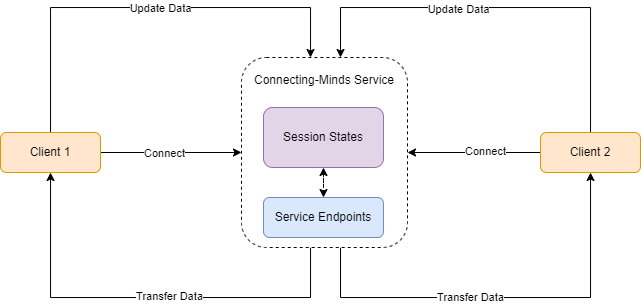
\includegraphics[width=1\linewidth]{content/pictures/CM-Archticture.png}
\caption{Connecting-Minds Infrastruktur (Quelle: eigene Darstellung)}
\label{fig:cm-topology}
\end{figure}

Nachdem eine Topologie bestimmt werden konnte (vgl. Abbildung \ref{fig:cm-topology}), muss nun bestimmt werden, auf welche Weise die Anwendungen im Detail miteinander kommunizieren. 

% Durch das \ac{OSI}-Modell 
Das \ac{OSI}-Modell zeigt auf, welche verschiedenen Schichten in der Netzwerkkommunikation durchlaufen werden können (vgl. \cite{noauthor_osi-modell_nodate}). Jede Netzwerkkommunikation zwischen Anwendungen muss dabei durch den Transport-Layer der jeweiligen Endgeräte gehen. Innerhalb dieser Transportschicht existieren einige Protokolle, die den Transport der versendeten Datenpakete übernehmen. Die am häufigsten verwendeten Protokolle sind dabei das \ac{UDP} und das \ac{TCP} (vgl. \cite{noauthor_transport_nodate}). 

\begin{figure}[ht]
\centering
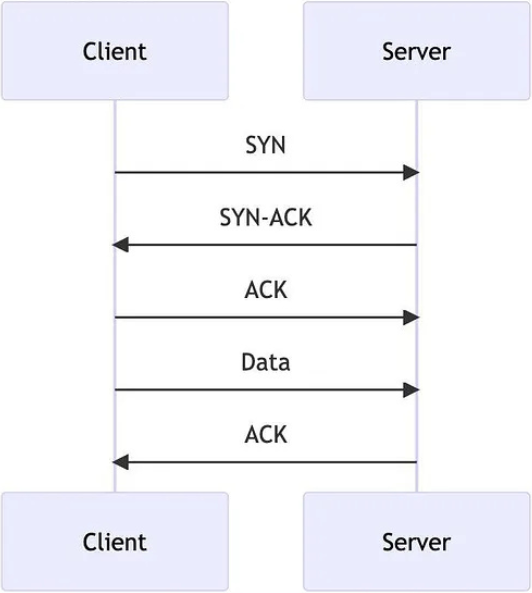
\includegraphics[width=0.5\linewidth]{content/pictures/TCP-Network.png}
\caption{Kommunikationsverbindung über TCP (Quelle: \cite{mygames_unity_2024})}
\label{fig:tcp}
\end{figure}

% Abbildung 
\ac{TCP} ist ein verbindungsorientiertes Protokoll, das zunächst eine Verbindung zu seinem Kommunikationspartner aufbaut, um Daten auszutauschen. Durch die Verbindung gewährleistet es einen zuverlässigen Datenaustausch, bei dem auch alle übertragenen Daten in der richtigen Reihenfolge beim Empfänger ankommen. Abbildung \ref{fig:tcp} zeigt diesen Verbindungsaufbau.
Zunächst erstellen der Client und Server einen Socket, um Daten über \ac{TCP} auszutauschen. Im Anschluss sendet der Client ein \ac{SYN}-Segment an den Server mit einem gewünschten Zielport. Anschließend akzeptiert der Server das \ac{SYN}-Segment, erstellt einen eigenen Socket und sendet an den Client ein \ac{SYN}-\ac{ACK}-Segment zurück. Der Client beantwortet dies mit einem \ac{ACK}-Segment. Nun besteht eine bidirektionale Verbindung  (vgl. \cite{mygames_unity_2024}).

% Einen \say{Distributed Authority} Ansatz kann es im Aufbau des Prototyps nicht gehebn
\ac{UDP} ist ein einfacheres Protokoll als \ac{TCP}, es garantiert weder die Zustellung noch die Reihenfolge der versendeten Pakete. Es baut zudem keine Verbindung zu seinem Kommunikationspartner auf, sondern sendet diese direkt an den Kommunikationsteilnehmer. Dadurch ist es wesentlich schneller als \ac{TCP} und wird häufig in Online-Spielen verwendet, die eine Echtzeitdatenübertragung erfordern (vgl. Abbildung \ref{fig:udp}). Da \ac{UDP} keine Zustellung garantiert, benötigt die Verwendung eine sorgfältige Handhabung (vgl. \cite{mygames_unity_2024}).

\begin{figure}[ht]
\centering
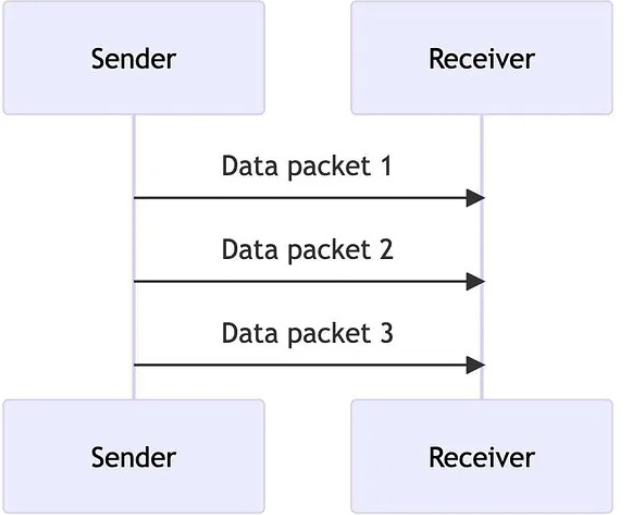
\includegraphics[width=0.5\linewidth]{content/pictures/UDP-Network.png}
\caption{Kommunikation über UDP (Quelle: \cite{mygames_unity_2024})}
\label{fig:udp}
\end{figure}

Auf Basis der Grundprotokolle \ac{TCP} und \ac{UDP} existieren auch Erweiterungen zu diesen. So ist das WebSocket Protokoll ein Application-Level Protokoll, das auf \ac{TCP} basiert. Es ermöglicht die Erstellung einer Verbindung zwischen zwei Kommunikationsteilnehmern (etwa einem Browser und seinem Server). Im Vergleich zum \ac{HTTP}-Protokoll ermöglicht es eine bidirektionale Kommunikation zwischen den Teilnehmern. So kann der Server seinen Clients Nachrichten senden, ohne dass zuvor eine \ac{HTTP}-Nachricht versendet wurde (vgl. \cite{mygames_unity_2024}).

\begin{figure}[ht]
\centering
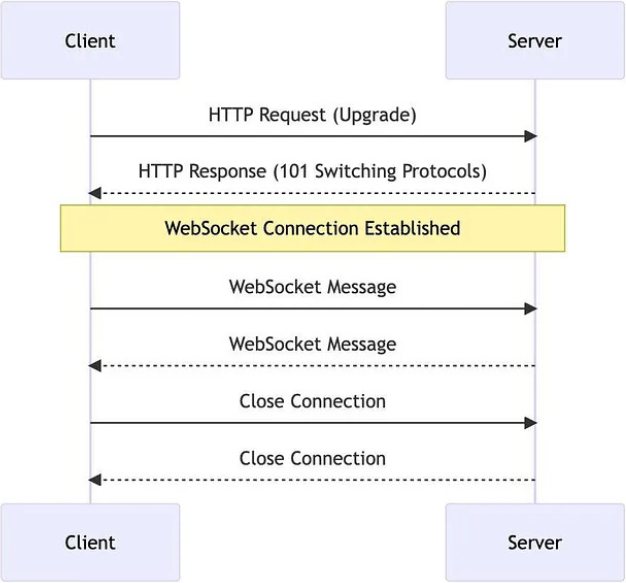
\includegraphics[width=0.5\linewidth]{content/pictures/WebSocket-Network.png}
\caption{Kommunikation über WebSocket (Quelle: \cite{mygames_unity_2024})}
\label{fig:ws}
\end{figure}

Für die entworfene Topologie ist die Kommunikation über das WebSocket-Protokoll das geeignetste. Es besteht eine persistente Verbindung der einzelnen verbundenen Anwendungen zum Server, welcher je nach Zustandsänderung an alle mit der Spielsitzung verbundenen Teilnehmer die Änderungen mitteilen kann. Dabei müssen sich die Teilnehmer nicht um eine Aktualisierung ihrer Zustände kümmern und erhalten zu jeder Zeit ein Update vom verbundenen Server (vgl. Abbildung \ref{fig:ws}).

\paragraph{Einbettung des Servers}

\begin{figure}[ht]
\centering
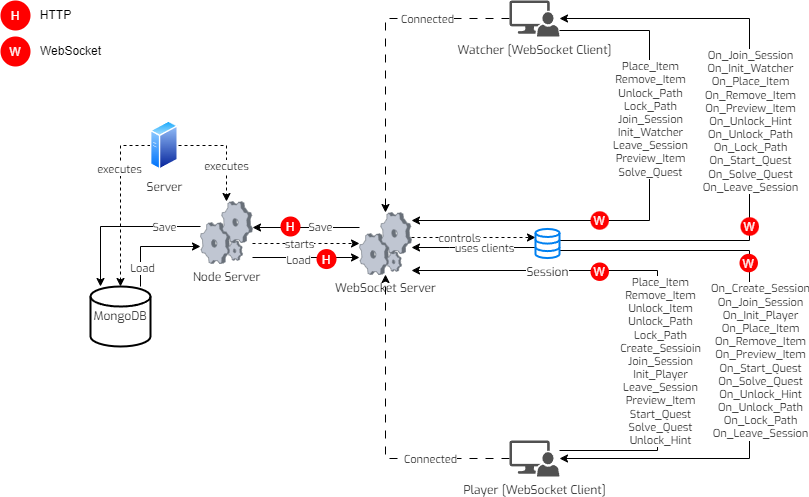
\includegraphics[width=1\linewidth]{content/pictures/Server-System.png}
\caption{Aufbau des Server (Quelle: eigene Darstellung)}
\label{fig:cm-server}
\end{figure}

Abbildung \ref{fig:cm-server} zeigt den Aufbau des Servers. Der physische Server führt dabei eine MongoDB Datenbank und einen Node-Server aus. Die MongoDB wird für die persistente Speicherung der einzelnen Sessions verwendet. Der Node-Server ist das Basis-Element der Server-Anwendung, da dieser den WebSocket Server startet, mit welchem sich die Spielteilnehmer verbinden werden. Der WebSocket Server ist zu dem dafür zuständig, dass durch die Aufforderung des Players neue Sessions erstellt werden. Wurde eine Session erstellt, wird der Player ihr automatisch beitreten. Ein Watcher kann nun ebenfalls der Session über den WebSocket Server beitreten. Die einzelnen mit dem Server verbundenen Clients kommunizieren nun über den Server mit der entsprechenden Session, welche über den Server Informationen zurückgibt. Die Clients kommunizieren dabei über das genannte WebSocket Protokoll.

Werden Sessions verlassen, werden diese vom WebSocket Server gespeichert. Dies geschieht durch \ac{HTTP}-Anfragen an den Basis Node-Server, welcher über seine Endpunkte die entsprechenden Daten abspeichert. Sie können durch Beitreten einer bereits existierenden Session wieder geladen werden. Senden Player als auch Watcher eine Beitritts-Anfrage an den WebSocket-Server, so lädt dieser über den Node-Server und den entsprechenden Endpunkt diese Session und lässt die Anfragenden sofern eine Session gefunden wurde, beitreten.

% \paragraph{Vorstellung der Datenmodelle}

\section{Herausforderungen in der Umsetzung}\label{sec:difficulties}
Die Umsetzung einer Spielidee stellt oft im Verlauf des Entwicklungsprozesses Hürden bereit, welche auf verschiedenste Weisen gelöst werden müssen. Auch diese Arbeit ist davon nicht verschont geblieben. So manche Herausforderungen mussten bewältigt werden.

\subsection{Erste Schritte im Leveldesign}
Zu Beginn der Schaffung der Spielwelt wurde überlegt, wie die Spielwelt auf einfache Weise gebaut werden kann, damit man sich hinterher nur noch überlegen muss, wie die enthaltenen Rätsel aussehen können. Um einzelne Spielräume generativ bauen zu können, wurde das Unity-Package von \cite{alasl_autolevel_nodate} näher betrachtet.

Das Asset umfasst einen Level-Builder, der aus den konfigurierten Modellen aus einem Repository generativ eine Spielwelt baut. Abbildung \ref{fig:level_builder} zeigt ihn in der Anwendung. Der Nutzer kann innerhalb des bestimmten Rasters einzelne Teile auswählen und dem Generator mitteilen, dass manche Stellen einen Hohlraum oder zusätzliche Elemente aus anderen Repositorys haben sollen.

\begin{figure}[ht]
\centering
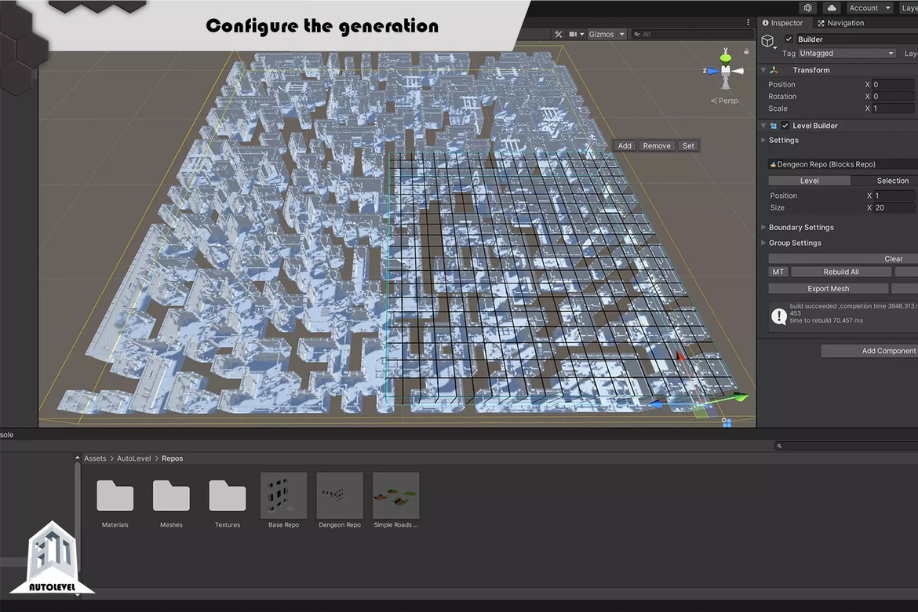
\includegraphics[width=1\linewidth]{content/pictures/FirstSteps00.png}
\caption{Level Builder Komponente (Quelle: \cite{alasl_autolevel_nodate})}
\label{fig:level_builder}
\end{figure}

Abbildung \ref{fig:level_builder_edit} zeigt dies anschaulich. Eine Teilfläche um das obere Ende des Level-Builder-Umfangs wurde über ein Menü des Builders ausgewählt und soll nun eine Anweisung für den Generator erhalten. In diesem Fall kann der Nutzer nun dem ausgewählten Bereich eine \say{Empty}Eigenschaft geben, sodass an dieser Stelle kein Raum generiert wird.

\begin{figure}[ht]
\centering
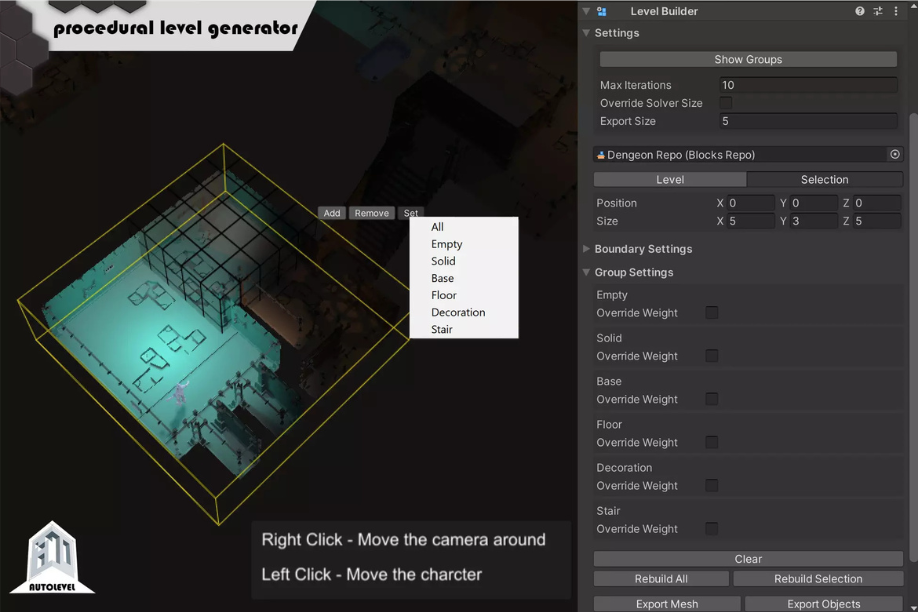
\includegraphics[width=1\linewidth]{content/pictures/FirstSteps01.png}
\caption{Level Builder Komponente (Quelle: \cite{alasl_autolevel_nodate})}
\label{fig:level_builder_edit}
\end{figure}

Um das Generieren der Spielwelt zu ermöglichen, muss zunächst ein Repository an Objekten erstellt werden, welche der Algorithmus verwendet. Ein Repository besteht aus einzelnen verschieden aussehenden 1x1x1 Meter großen modulare Einzelteile, die über das in Abbildung \ref{fig:repository-generator} gezeigte Menü zusammengesteckt werden können. So können aus den sechs Einzelteilen in der Abbildung viele verschiedene 2x3 große Teile ergeben, welche der Level Builder generieren kann.

\begin{figure}[ht]
\centering
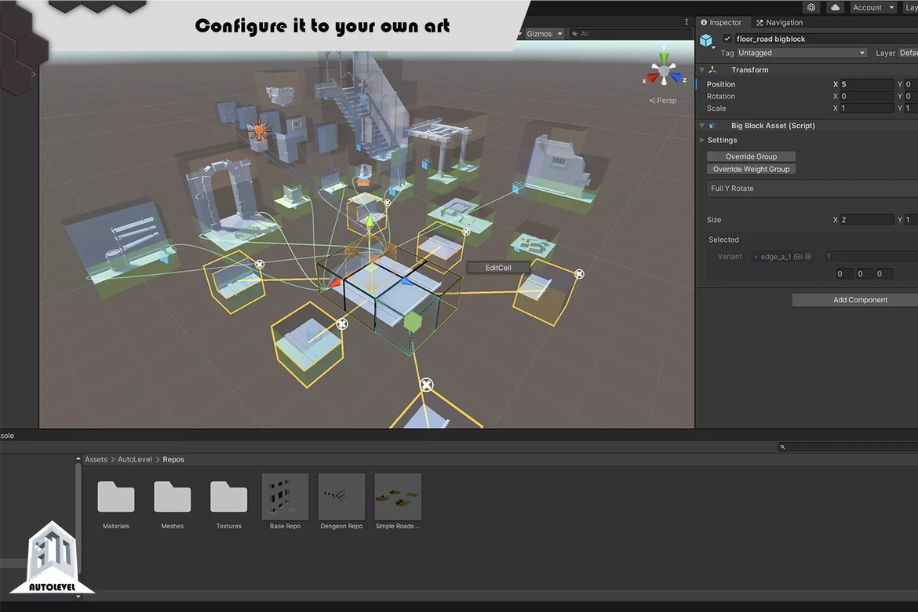
\includegraphics[width=1\linewidth]{content/pictures/FirstSteps02.png}
\caption{Level Builder Komponente (Quelle: \cite{alasl_autolevel_nodate})}
\label{fig:repository-generator}
\end{figure}

Dieses Paket setzt allerdings voraus, dass jedes Struktur gebende \ac{3D}-Objekt in seine 1x1x1 Meter große Basis zerlegt wird. Das wäre bei Assets, die über den Asset-Store hinzugenommen wurden, ein viel zu großer Aufwand geworden.

Daher wurde nach einem Generator geschaut, der fertige Strukturelemente wie Boden-Modelle oder Wand-Elemente verwenden kann. \cite{mysticforge_low_nodate} stellt einen Generator bereit, bei dem für verschiedene Abschnitte, wie Links/ Rechts Kurven, zweier oder dreier Kreuzungen oder geraden Stücken, verschiedene Varianten bereitgestellt werden können und der Generator aus diesen eine Spielwelt generiert. Zusätzlich konnten auch angefertigte Räume mit bereitgestellt werden, in welchen im späteren Verlauf die Rätsel eingebaut werden können. Die Elemente, die zwischen diesen Räumen generiert wurden, können so als Verbindungsstücke dienen, durch welcher der Watcher den Player navigieren müsste. Auch dieser Generator benötigt Modelle in einer bestimmten Größen-Norm. Diese ist jedoch im Vergleich zum Generator von \cite{alasl_autolevel_nodate} nicht zu kleinteilig und bezieht sich auf strukturgebende Elemente wie Wände als Ganzes.

\begin{figure}[ht]
\centering
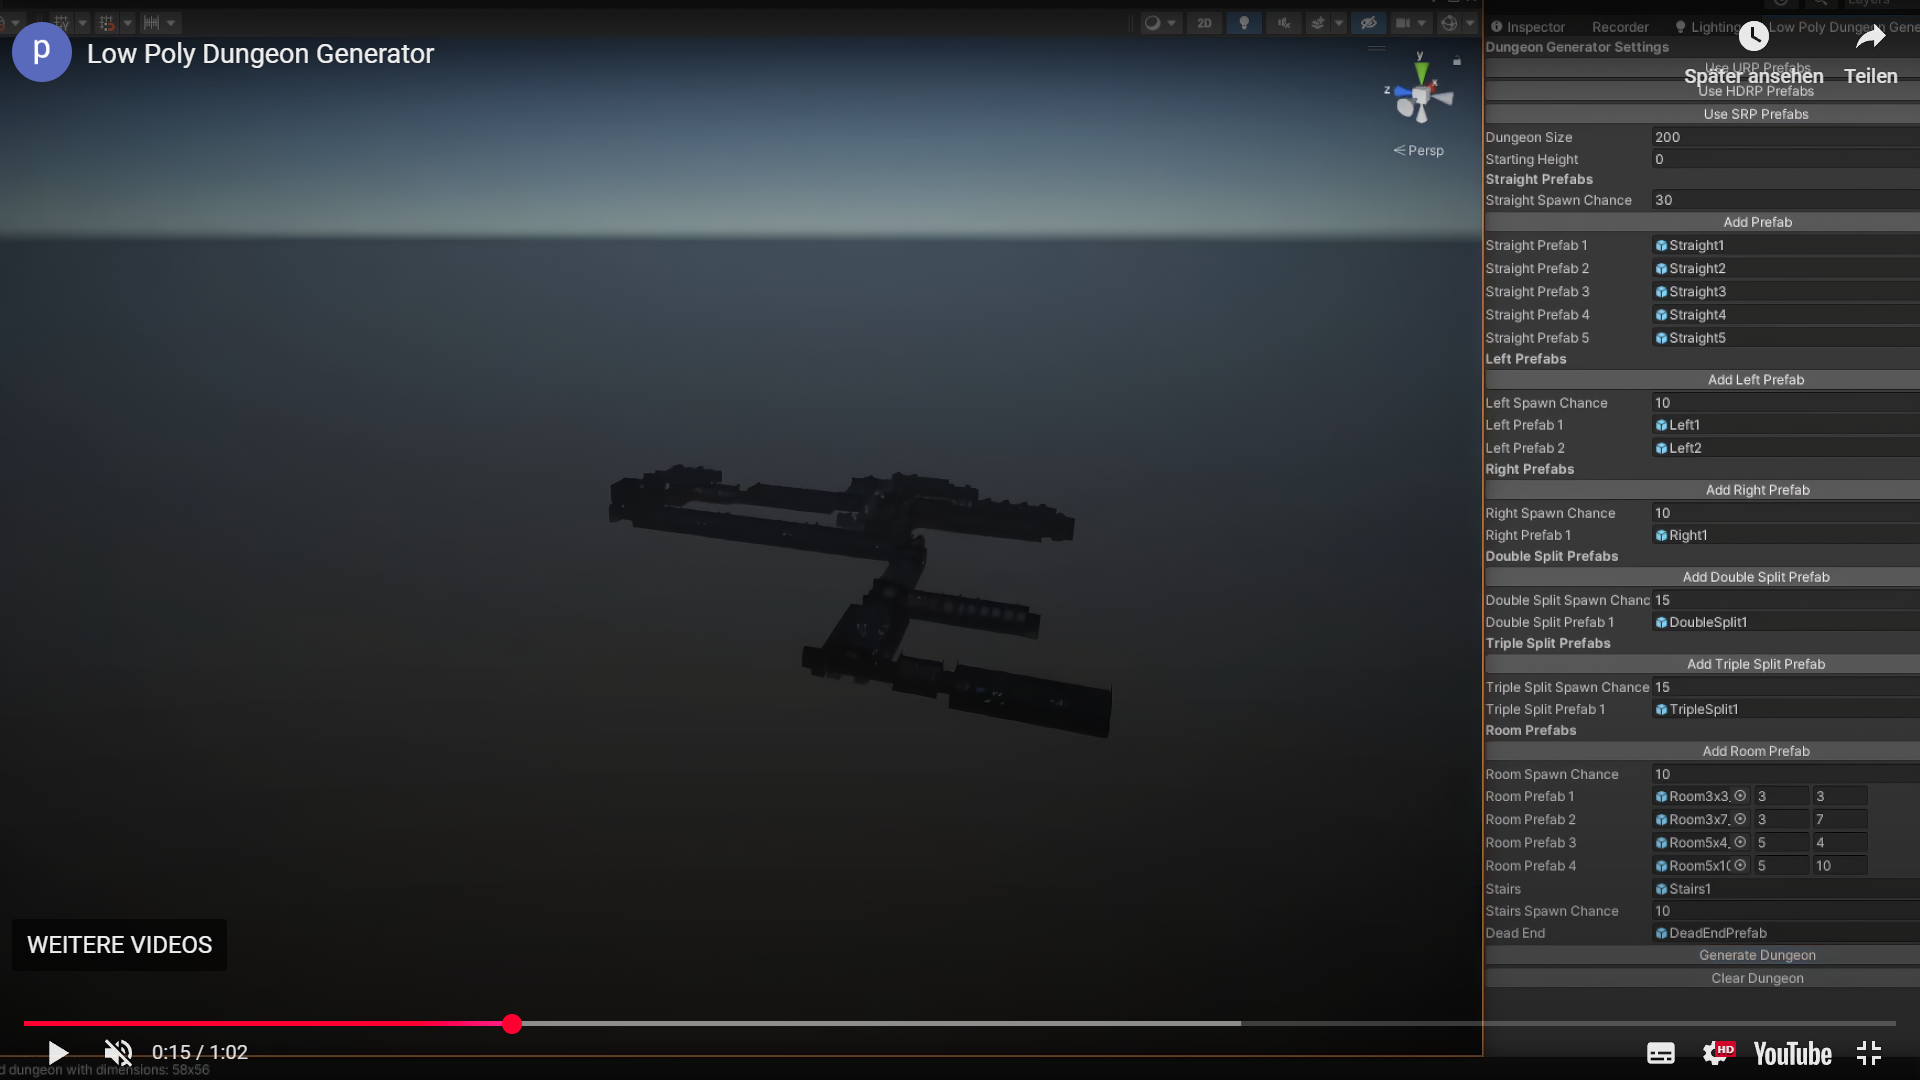
\includegraphics[width=1\linewidth]{content/pictures/FirstSteps03.png}
\caption{Low-Poly Dungeon Generator (Quelle: \cite{past12pm_low_2024})}
\label{fig:dungeon-generator}
\end{figure}

Leider werden die verschiedenen Elemente zufällig hintereinander gereiht. Deshalb wurde der Ansatz aus dem vorangegangenem Generator mit eingebaut. So konnte nun bestimmt werden, welche Objekte auf welche Folgen und welche zuvor kommen sollen. Abbildung \ref{fig:athaeck-dungeon-generator} zeigt das Ergebnis aus den in einer in Norm erstellten Strukturelementen (oberes Bild) generierte Wege zwischen den Räumen (unteres Bild). Es ist nun so, dass durch das Zufallsprinzip, zu welcher Wahrscheinlichkeit wann welche Elemente kommen, zu viel Unruhe entsteht und das Ergebnis so für den Anwendungszweck nicht nutzbar ist.

\begin{figure}[ht]
\centering
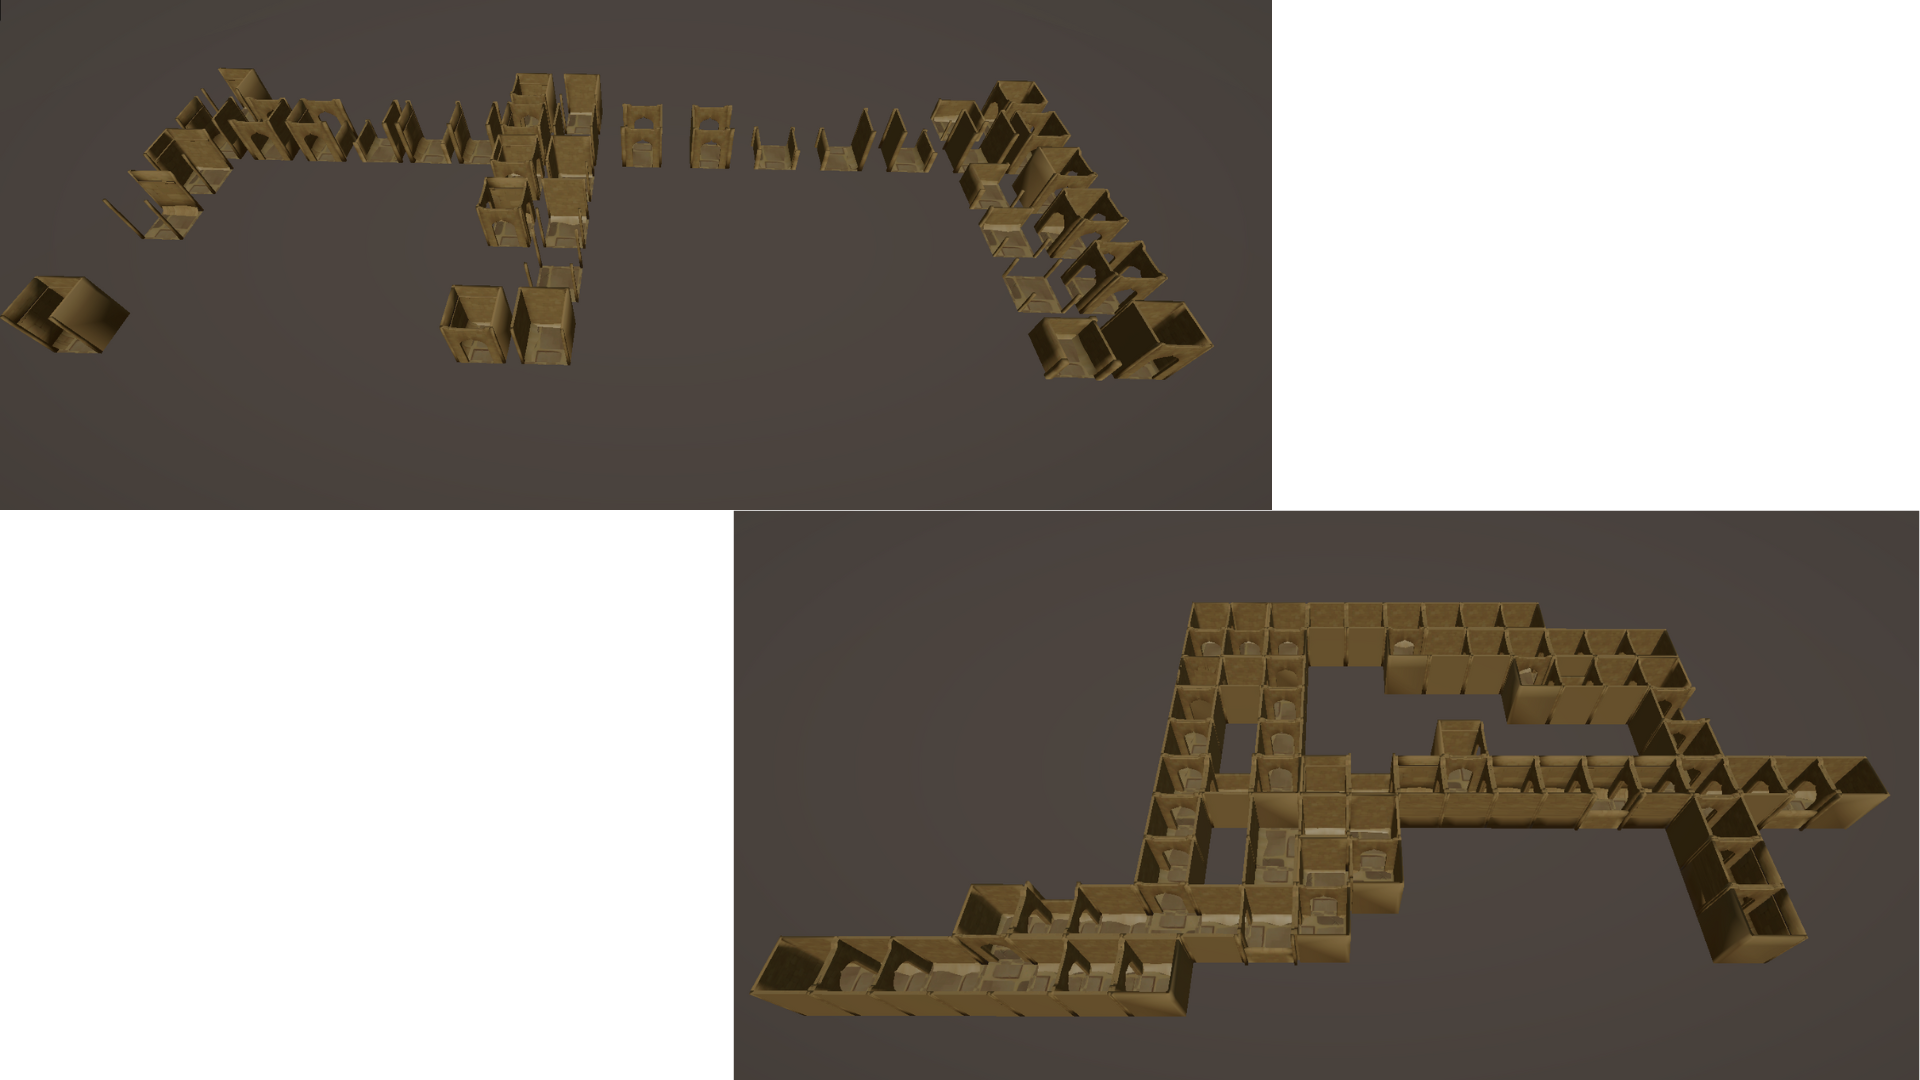
\includegraphics[width=1\linewidth]{content/pictures/FirstSteps06.png}
\caption{athaeck Dungeon Generator (Quelle: eigene Darstellung)}
\label{fig:athaeck-dungeon-generator}
\end{figure}

Jedoch hatte dieser nicht weitergeführte Ansatz auch ein positives Ergebnis. Da die einzelnen Elemente der Strukturelemente in einer bestimmten selbst definierten Norm angepasst werden mussten, konnte im weitere Verlauf das Leveldesign mit diesen Maßstäben die weiteren hinzugenommenen Assets angepasst und verwendet werden.

\subsection{Physik-System von Unity}\label{sec:unity-physics-system}
Die Kern-Mechanik des Lösens von Hindernissen in diesem Prototyp ist das Platzieren von Gegenständen an bestimmte Stellen. Zu einem ???? gibt es auch einn andren Teil???? Teil werden die Platzierungen der Objekte über das Physik-System von Unity überprüft. Jeder platzierte Gegenstand besitzt einen Collider, der auf Kollisionen mit anderen Collidern, wie dem des Player-Avatars reagiert. Wie in den Beispielen der \say{QuestSolver} (vgl. Abschnitt \nameref{sec:quest-system}) oder \say{PathActivator} (vgl. Abschnitt \nameref{sec:path-system}) reagieren nun diese Komponenten auf die Collider der Gegenstände, die innerhalb der eigenen Collider platziert werden (vgl. Abbildung \ref{fig:collision-sketch}). 

% [TODO: Zur veranschaulichung eine Zeichnung eimbauen?]
\begin{figure}[ht]
\centering
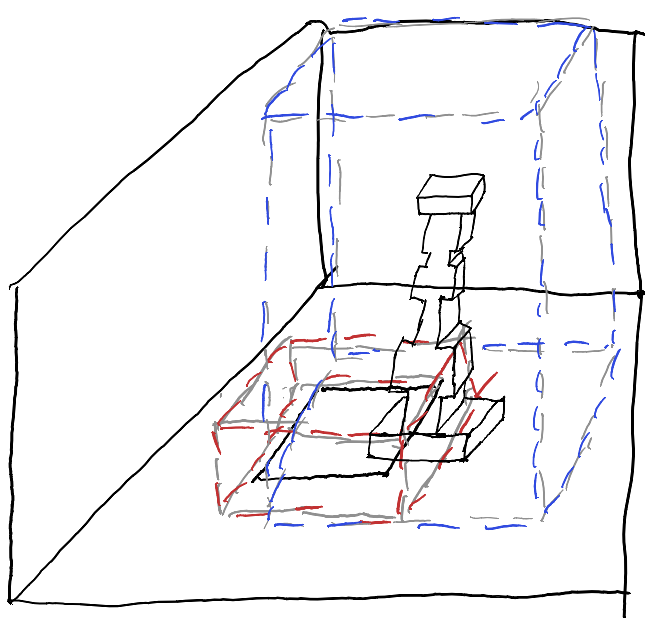
\includegraphics[width=.6\linewidth]{content/pictures/CollisionSketch.png}
\caption{Kollision zweier Collider in dem Raum, bei dem blau und rot sich kreuzen (Quelle: eigene Darstellung)}
\label{fig:collision-sketch}
\end{figure}


Sobald ein Gegenstand innerhalb eines anderen Colliders platziert wird, errechnet das Physik-System eine Kollision, welche in den gehandhabten Klassen nun empfangen werden kann. Das \say{Script lifecycle flowchart} von Unity in \cite{technologies_unity_nodate} zeigt dies anschaulich. Nachdem ein neuer Knoten in die Spielwelt instanziiert wurde, beginnt zunächst die Initialisierung der enthaltenen Skripte. Anschließend erfolgt die Errechnung des Physik-Systems, ehe es weiter über Input-Events und die Spiellogik geht.

Es gab jedoch Probleme beim Entfernen der einzelnen Objekte aus den genannten Zielradien der Collider. Der Lebenszyklus von Unity errechnet, nachdem ein Gegenstand entfernt wurde, keine physikalischen Veränderungen des entfernten Objekts (in der Abbildung nach \say{OnApplicationQuit} zu sehen). Für das Lösungssystem der Hindernisse und der Aktivierung oder Deaktivierung von bestimmten Pfaden ist dies ein Problem.

Aus diesem Grund wurde eine Basisklasse geschrieben, die an den zur Laufzeit hinzugefügten und entfernten Objekten liegt. Von ihr aus sollen nun Kollisionen ausgeführt werden. In der Vergangenheit wurde jeweils an den Objekten, die die Kollisionen empfangen, diese behandelt. Zum Teil bleibt dieses Prinzip erhalten, allerdings ist diesmal der Verursacher auch derjenige, der zur Laufzeit entfernt wird.

\begin{figure}[ht]
\centering
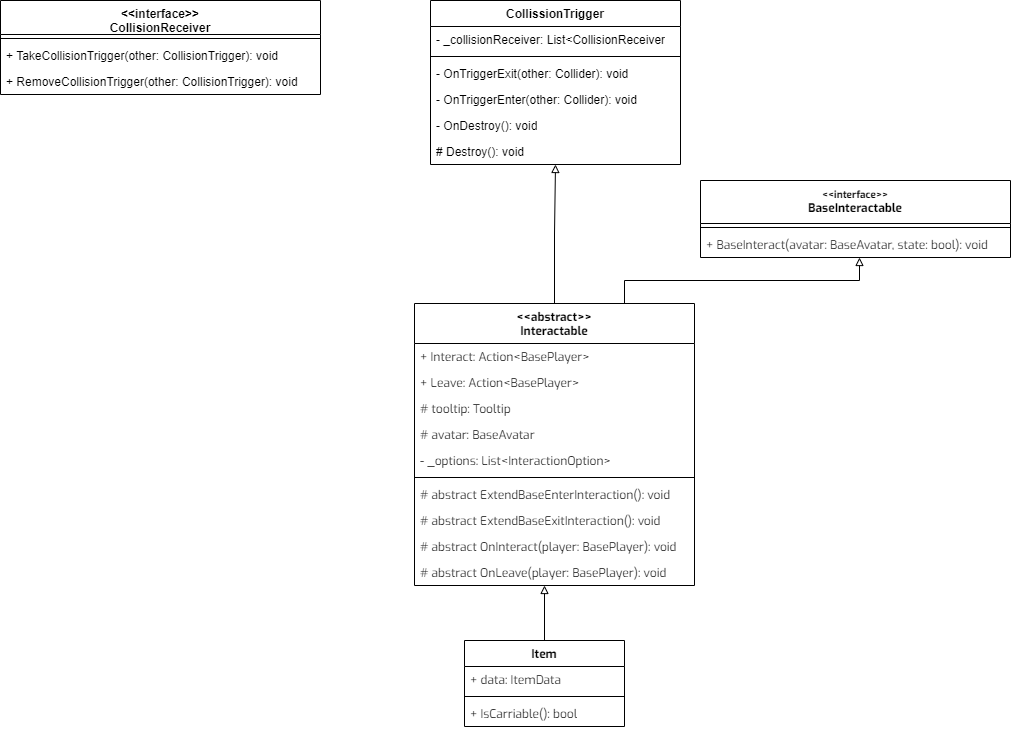
\includegraphics[width=1\linewidth]{content/pictures/CollisionSystem.drawio.png}
\caption{Neue Herangehensweise an Kollisionen (Quelle: eigene Darstellung)}
\label{fig:new-collision-system}
\end{figure}

Abbildung \ref{fig:new-collision-system} zeigt die neue Klasse des \say{Verursachers} von Kollisionen (in letzter Vererbungs-Stufe das \say{Item}-Skript, welches am Gegenstandobjekt liegt, welches platziert wird) und das Empfänger-Interface, das nun wie in Abbildung \ref{fig:new-collision-system-in-quests} von der \say{BasePlaceableActivator} Basis-Klasse vererbt wird. 

\begin{figure}[ht]
\centering
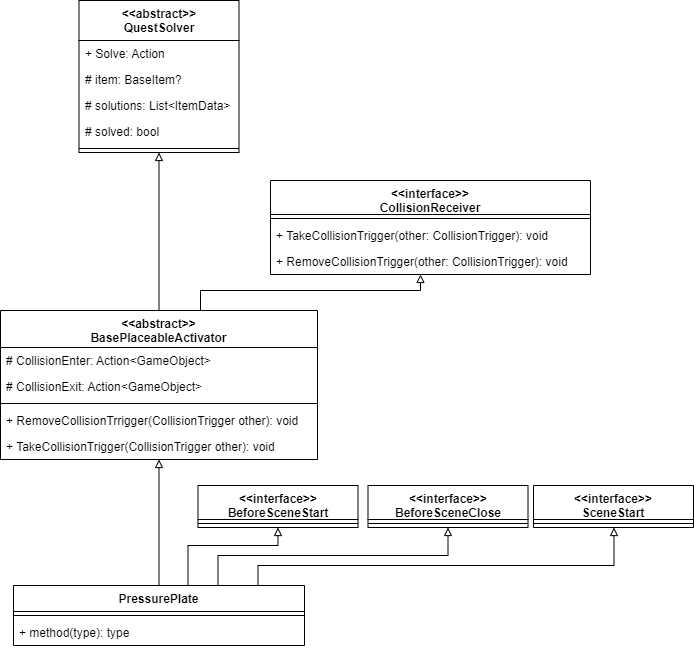
\includegraphics[width=0.8\linewidth]{content/pictures/Quest-Extension.drawio.png}
\caption{Kollisions-Empfänger im Quest-System (Quelle: eigene Darstellung)}
\label{fig:new-collision-system-in-quests}
\end{figure}

\subsection{Platzieren von Gegenständen außerhalb der Spielwelt}\label{sec:difficulties-placement}
Wie bereits erwähnt, besitzen der Player und der Watcher zum Teil unterschiedliche Ansichten der Räume. Am Beispiel des Sicherheitsraumes wird das folgende Problem, das Platzieren von Gegenständen mit sich führen kann, vorgestellt. 

Im Sicherheitsraum befindet sich der Player innerhalb des Gebäudes, wohingegen der Watcher zusätzlich einen kleinen Außenbereich sieht, auf den er einen gefundenen Stromgenerator platzieren muss. Da sich für den Watcher dieser Bereich geöffnet hat, kann er den Generator auf diesem Bereich ohne Probleme platzieren. Da jedoch alle in der Session platzierten Gegenstände sowohl beim Watcher als auch beim Player platziert werden, stößt dies auf ein Problem. Der Player darf keine Gegenstände sehen, welche in nicht aktiven Bereichen liegen. 

Aus diesem Grund wurde für jeden Bereich Collider in die Spielwelt platziert, die dafür verantwortlich sind, Gegenstände zu aktivieren oder zu deaktivieren, je nachdem, ob der Bereich aktiv oder inaktiv ist. Das umgeänderte System aus dem vorangegangenen Kapitel \nameref{sec:unity-physics-system} und die Klasse \say{PathCollider} aus dem Kapitel \nameref{sec:path-system} spielen hier dabei zusammen und ermöglichen es, dass sowohl Player als auch Watcher keine \say{falschen} Objekte außerhalb der aktiven Weltgebiete sehen können.

Jedoch fielen in der Evaluation der Anwendungen Grenzfälle auf, die im Kapitel \nameref{sec:prospect} weiter behandelt werden.



% erste Ansätze im Levelbuilding erwähnen

% hier kommt das placing also die positionen in der spielwelt

% dann drauf bezogen das mit den slots, dass die ne position haben später auch fürs setzen wichtig
% das mit den collidern, was man auch anders umsetzen kann noch, das noch erwähnen






% bei umsetzung müssen die 3d und ar anwendung vorgestellt werden vom watcher
% hier muss ein bezg auf das paper mit den steuerungen für touch erwähnt werden


% die anwendung vom playewr

\section{Probleme in der Umsetzung}
Für die Evaluation war geplant, dass die Anwendung des Watchers über eine \ac{AR}-Integration verfügt. Ein Kernelement einer funktionierenden \ac{AR}-Anwendung ist das Platzieren des entsprechenden \ac{3D}-Objektes in den virtuellen Raum, der durch die Sicht des Smartphones aussieht, als wäre er im echten Raum platziert. Damit das Platzieren des Weltobjektes der Anwendung des Watchers auch gut verankert ist, wurde das \say{Place detection}-Modul der \ac{AR}Foundation verwendet. Zusätzlich wurden auf der ausgewählten Plane ein \ac{AR}Anchor platziert, welcher mit Hilfe des Anchor-Managers ein zuverlässigeres Platzieren \ac{AR} gewährleisten soll.

Das Ergebnis, das dabei heraus kam war, dass sich die platzierte Spielwelt in einem bestimmten Abstand zur Kamera immer mitbewegt hat. Zu sehen ist dies ebenfalls in diesem Unity-Forum im vorletzten Beitrag von Howard258 \cite{noauthor_unity_2025}. Es wurden einige Lösungsversuche, wie das Umstellen der Zuordnung in der Anchor und Plane Platzierung, oder das Umstellen der Weltknoten, versucht. Jeder neue Ansatz brachte leider keine Lösung für das Platzierungsproblem. In einem weiteren Forum (vgl. \cite{noauthor_ar_2023}) wurde gezeigt, dass die genutzte Version der \ac{AR}Foundation und der Unity-Editor Version ein Grund für die deffekte \ac{AR}-Platzierung ist. Dieser Lösungsweg wurde aus zeitlichen Gründen nicht mehr umgesetzt, da eine Versions-Änderung des Editors und seine enthaltenen Assets auch zu weiteren Problemen führen könnten. 

Ebenfalls wurde auch keine weitere Platzierungsmethode wie das \say{Image tracking} verwendet, da sich der Watcher frei in seiner physischen Welt bewegen soll und die Gefahr besteht, dass das Vergleichsbild nicht mehr gesehen wird und der Spieler keine Spielwelt mehr vor sich sieht.
% AR

% Gerätefindung im selben Netzwerk -> eher Herausforderungen in der Evaluation